\documentclass{book}

% vim:set errorformat="":
\usepackage{amsmath}
\usepackage{amsfonts}
\usepackage{amssymb}
\usepackage{xcolor}
\usepackage{colortbl}
\usepackage{marginnote}
\usepackage{wrapfig}
\usepackage{graphicx}
\usepackage{lipsum}
\usepackage{array}
\usepackage{tabularx}
\usepackage{environ}
\usepackage{bussproofs}
\usepackage{exercise}
\usepackage{imakeidx}
\usepackage[normalem]{ulem}
%\usepackage{fontspec} % xelatex only
\usepackage{hyperref} % must be the last one
\hypersetup{
    colorlinks=true,
    linkcolor=blue,
    citecolor=blue,
    urlcolor=blue
}
\renewcommand{\ExerciseHeader}{\medskip\noindent\textbf{\ExerciseName~\ExerciseHeaderNB.~\ExerciseHeaderDifficulty}\emph{\ExerciseHeaderTitle}\\~\\}
\renewcommand{\AnswerHeader}{\medskip\noindent{\textbf{Answer of \ExerciseName~\ExerciseHeaderNB}\\}}

\usepackage[skins,listings]{tcolorbox}
\usepackage{boolexpr,ifthen}
\definecolor{dkblue}{rgb}{0,0.1,0.5}
\definecolor{lightblue}{rgb}{0,0.5,0.5}
\definecolor{dkgreen}{rgb}{0,0.4,0}
\definecolor{dk2green}{rgb}{0.4,0,0}
\definecolor{dkviolet}{rgb}{0.6,0,0.8}
\definecolor{mantra}{rgb}{0.2,0.6,0.2}
\definecolor{gotcha}{rgb}{0.8,0.2,0}

\def\lstlanguagefiles{defManSSR.tex}
\lstset{language=SSR}
\newcommand{\mcbimpl}[1]{\lstinline/?$_{#1}$/}
\newcommand{\mcbimplm}[1]{\mbox{?}_{#1}}

\newcommand{\lib}[1]{\textsf{#1}}

\newcommand{\C}[1]{\mbox{\lstinline`#1`}}
\newcommand{\D}[1]{\mbox{\lstinline'#1'}}
\let\L=\lstinline

% Highlights identifiers, |* id *| in underlined red, can we do better?
\lstset{moredelim=[is][\color{red}\bfseries\ttfamily\underbar]{|*}{*|}}
\lstset{moredelim=[is][\ttfamily\uwave]{|==}{==|}}
\lstset{moredelim=[is][\ttfamily\underbar]{|--}{--|}}

\newcommand\Chapter[2]{\chapter
  [#1\hfil\hbox{}\protect\linebreak{\itshape#2}]
  {#1\\ [2ex] {\Large \itshape #2}}
  \markboth{\MakeUppercase{\chaptername\ \thechapter.\ #1}}{}}

\newcolumntype{V}{>{\centering\arraybackslash} m{0\linewidth} }

\newcommand{\gotcha}[1]{
\begin{center}
\begin{tcolorbox}[colframe=gotcha,
	center title,
	title={\textcolor{white}{\textsf{\Large\textbf{Warning}}}}]
\begin{tabular}{lV}
\begin{minipage}{0.86\textwidth}
\vspace{1em}
#1
\end{minipage}
&
\warnsign{1cm}
\end{tabular}
\end{tcolorbox}
\end{center}}

\newcommand{\mantra}[1]{
\begin{center}
\begin{tcolorbox}[colframe=mantra,
	center title,
	title={\textcolor{white}{\textsf{\Large\textbf{Advice}}}}]
\begin{tabular}{lV}
\begin{minipage}{0.86\textwidth}
\vspace{1em}
#1
\end{minipage}
&
\coqhead{1cm}
\end{tabular}
\end{tcolorbox}
\end{center}}

\newcommand{\coqhead}[1]{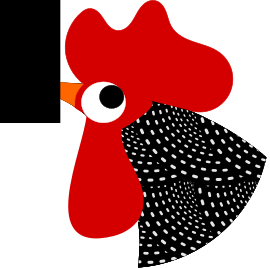
\includegraphics[width=#1]{../artwork/smallpantade}}
\newcommand{\warnsign}[1]{\includegraphics[width=#1]{../artwork/Ambox_warning_pn}}

\newcommand{\mcbpplevel}[1]{
\switch[#1=]
\case{1}
\case{2} \hspace{0.6cm} \coqhead{0.6cm}
\case{3} \coqhead{0.6cm} \coqhead{0.6cm}
\otherwise Please use \textbackslash mcbLEVEL
\endswitch
}
\newcommand{\mcbpptxtlevel}[1]{
\switch[#1=]
\case{1}
\case{2} $(\star)$
\case{3} $(\star\star)$
\otherwise Please use \textbackslash mcbLEVEL
\endswitch
}


\newcommand{\mcbvarreset}{
\mcbLEARN{Please use \textbackslash mcbLEARN}
\mcbREQUIRE{Please use \textbackslash mcbREQUIRE}
\mcbPROVIDE{Please use \textbackslash mcbPROVIDE}
\mcbNOTES{}
\mcbLEVEL{4}}

\newcommand{\mcbLEARN}[1]{\def\mcbvarLEARN{#1}}
\newcommand{\mcbREQUIRE}[1]{\def\mcbvarREQUIRE{#1}}
\newcommand{\mcbPROVIDE}[1]{\def\mcbvarPROVIDE{#1}}
\newcounter{mcbvarLEVEL}
\newcommand{\mcbLEVEL}[1]{\setcounter{mcbvarLEVEL}{#1}}
\newcommand{\mcbNOTES}[1]{\def\mcbvarNOTES{#1}}
\newcounter{mcbvarTMP}

\newcommand{\mcbsection}[1]{
\setcounter{mcbvarTMP}{1}
\ifthenelse{\equal{}{\mcbvarNOTES}}{\setcounter{mcbvarTMP}{0}}{}
\section[#1 \mcbpptxtlevel{\value{mcbvarLEVEL}}]{#1}
\smash{\raisebox{0.7cm}{\hspace{0.92\textwidth}\mcbpptxtlevel{\value{mcbvarLEVEL}}}}
%\marginnote{\small\begin{tabular}{p{3.8cm}}\hline
%\textbf{Learns} \mcbvarLEARN \\
%\textbf{Requires} \mcbvarREQUIRE \\
%\textbf{Provides} \mcbvarPROVIDE \\
%\textbf{Level} \arabic{mcbvarLEVEL} \\
%\switch[\value{mcbvarTMP}=]
%\case{0}
%\case{1} \textbf{Note} \mcbvarNOTES \\
%\endswitch
%\hline
%\end{tabular}\\~\\
%}
\mcbvarreset{}
}

\newcommand{\mcbsubsection}[1]{
\setcounter{mcbvarTMP}{1}
\ifthenelse{\equal{}{\mcbvarNOTES}}{\setcounter{mcbvarTMP}{0}}{}
\subsection[#1 \mcbpptxtlevel{\value{mcbvarLEVEL}}]{#1}
\smash{\raisebox{0.7cm}{\hspace{0.92\textwidth}\mcbpptxtlevel{\value{mcbvarLEVEL}}}}
%\marginnote{\small\begin{tabular}{p{3.8cm}}\hline
%\textbf{Learns} \mcbvarLEARN \\
%\textbf{Requires} \mcbvarREQUIRE \\
%\textbf{Provides} \mcbvarPROVIDE \\
%\textbf{Level} \arabic{mcbvarLEVEL} \\
%\switch[\value{mcbvarTMP}=]
%\case{0}
%\case{1} \textbf{Note} \mcbvarNOTES \\
%\endswitch
%\hline
%\end{tabular}\\~\\
%}
\mcbvarreset{}
}


\newcommand{\mcbsubsubsection}[1]{
\setcounter{mcbvarTMP}{1}
\ifthenelse{\equal{}{\mcbvarNOTES}}{\setcounter{mcbvarTMP}{0}}{}
\subsubsection[#1 \mcbpptxtlevel{\value{mcbvarLEVEL}}]{#1}
\smash{\raisebox{0.7cm}{\hspace{0.92\textwidth}\mcbpptxtlevel{\value{mcbvarLEVEL}}}}
%\marginnote{\small\begin{tabular}{p{3.8cm}}\hline
%\textbf{Learns} \mcbvarLEARN \\
%\textbf{Requires} \mcbvarREQUIRE \\
%\textbf{Provides} \mcbvarPROVIDE \\
%\textbf{Level} \arabic{mcbvarLEVEL} \\
%\switch[\value{mcbvarTMP}=]
%\case{0}
%\case{1} \textbf{Note} \mcbvarNOTES \\
%\endswitch
%\hline
%\end{tabular}\\~\\
%}
\mcbvarreset{}
}
\mcbvarreset{}

\newbox{\devnull}
\NewEnviron{coqdef}[1]{}

\newcommand{\coqrun}[2]{}

\newtcblisting[auto counter]{coq}[2]{
	listing engine=listings,
	listing options={numbers=left,numberstyle=\tiny,
	                 aboveskip=0mm,belowskip=0mm,
		         xrightmargin=0mm,xleftmargin=0mm},
	%on line,
	before={\noindent},
	after={\hfill},
	listing only,
	fonttitle=\small\sffamily,%\bfseries,
	boxrule=0.2mm,top=1mm,bottom=1mm,
	#2
}
\newtcblisting{coqout}[2]{
	listing engine=listings,
	listing options={aboveskip=0mm,belowskip=0mm,
	                 xrightmargin=0mm,xleftmargin=0mm},
	%on line,
	before={\noindent},
	after={\hfill},
	listing only,
	fonttitle=\small\sffamily,%\bfseries,
	boxrule=0.2mm,top=1mm,bottom=1mm,
	#2
}

\newcommand{\Coq}{\textsc{Coq}}
\newcommand{\mcbCIC}{Calculus of Inductive Constructions}


\title{The Book}
\author{Assia, Enrico, \ldots (you are welcome)}

\begin{document}
\maketitle
\tableofcontents{}

\setcounter{chapter}{-2}
\chapter{Conventions}

Words:\\
\begin{tabular}{ll}
used & unused \\\hline
implicit argument, place holder & existential/meta variable \\
language of canonical structures & hints \\
declarative program & logic program \\
type inference & pretyping, elaboration \\
\end{tabular}



\setcounter{chapter}{-1}
\chapter{The essence of math comp}

\section{challenges faced and tools adopted}
(tools in a broad sense, the logic is a tool, coq is a tool, the plugin
is a tool, the ssr style is a tool,...)

Challenges:
\begin{itemize}
\item large body (scale up), make proofs small and robust.
	We need to say that we do use "deterministic automation".
	Use Laurent's data on de bruijn factor.
\item model the use of math notations, their role in proofs, model proofs (also
	it is about reasoning, not just computations). Another way to say that
	is: model Bourbaki (rationalization of Math via structure/interfaces)
	but not the first book (set theory) that is replaced by CIC (link with
	section computational thinking).
\end{itemize}

We build on Coq and an extension.  The main tools follow (in random order):

\section{Computational Thinking}\label{ch:compthink}

This section should motive the activity of formalizing mathematics
with the {\bf Coq} proof assistant, emphasizing its computing skills,
and as opposed to other foundations like HOL. However the challenge is
to keep mathematicians as the privileged target, while motivating the
ssr approach to a CS oriented reader.

See \verb+../coq/ch0.v+.

Aim of the chapter:
\begin{itemize}
\item should sound natural and easy to a CS person (but with the ssr twist)
\item should sound different but well motivated to a Coq user (do show, maybe in
  the exercises, that leqn is 100 times better than "Inductive le").  Try to
  reproduce the shock we had the first time we used Boolean predicates.  It may
  help to compare, in the *advanced* section, the approach with the standard
  one, so that one sees two proof scripts in the same page.
\end{itemize}

\section{logic programming ... type inference}
to model proof search, give a meaning to notations, teach coq the
work an informed reader does (contextualizing otherwise ambiguous
notations, knowledge of interface/instance of algebraic structures).

relation with proof search: no "blind" proof search (easy, ad-hoc, pervasive
v.s. advanced, generalistic, potentially expensive and unstable).

\section{automation in tactics}
the main points:
\begin{itemize}
\item 1/3 is rewrite, term selection/search (one does not need to reach a sub
	formula as a goal in order to make progress for example, no monkey
	puzzle as in GG terminology).
\item Create a formula without writing it: some advanced forms of forward
	reasoning tactics to deal with symmetries, generalizations (boils down
	to syntesize the cut formula out of the minimum possible user input, as
	in a text where one says "similarly to that, we can also prove that".
	(this is not very pervasive, dunno if it is worth putting it here in
	this chapter).  Also elim does that. (technically also rewrite, but we
	may want to separate things)
\end{itemize}
This section is were one talks about the plugin, and some of the main design
points of tactics: compositional (a language, not a list of commands),
predictable (documented!!!), finally compact (symbols for uninteresting steps).

\section{discipline}
MAKE an howto out of that.
Maybe one should also add a few notes on the style in scripts? like:
\begin{itemize}
\item you must be able to model (at least) 1 proof step in a sentence (line),
  e.g. "rewrite preparegoal dostep ?cleanup."
\item uninteresting/recurrent lemmas/steps should be small (short names, easy to
  gray out)
\item lemma statements are designed, not just written, having in mind their use
      (forward, backward, implicit argumets, arguments order)
      and the class of trivial hypotheses since an extra hyp that is proable
      triviality (via //, hint resolve, cnaonical) is for free. E.g.
      "x \\is a toto", "0 <= n", ...
\item also not every possible lemma, but a few that combine well
\item proofs/definitions are reworked many times, why (understand recurrent
  proof schemas, compact, factor, make more stable/robust) and what is needed
  (like meaningful names, clear structure)
\end{itemize}

\section{trivial=implicit (for a trained mathematician)}
The idea is to try to identify what is trivial (mathematically speaking)
and be sure you can model it as such:
\begin{itemize}
\item (level basic) make explicit the trivialities of each theory (what one
	expects to be proved by //). 
\item (level advanced) when you do new stuff, you must decide what is
	trivial/implicitly proved.
\item (hard) which technique to make Coq prove it automatically (hint resolve,
	canon, comput... in the type)
\end{itemize}

This may also be another way present the whole chapter

\mantra{(basic) if you see toto=false you should perform the case analysys via fooP}


\part{The art of formalizing}


\chapter{Programming}

Find a more catchy title? The motivation is: how to define things:
objects, operations, (boolean) relations.

Theoretical content:
\begin{itemize}
\item Functions with simple types ($\lambda$, $\rightarrow$)
\item Inductive {\bf datas}
\item Programs by case analysis and recursion
\item Compute
\item Polymorphic datatypes (introduce $\Pi$, and its \Coq{} notation
  \C{forall}, for quantification over datatypes only)
\item Everyone has a type : \C{0 : nat : Type : Type}
\end{itemize}
This is more or less a standard introduction to (a flavor of)
functional programming, with two possible difficulties:
\begin{itemize}
\item Be precise but not too technical (e.g. on inductive types)
\item Find a line of speech which does not bore/discourage
  mathematicians.
\item Somehow the syntax of (this fragment of the) terms should made
  be clear and precise.
\end{itemize}

\Coq{} commands and features:
\begin{itemize}
\item Implicit arguments (only to go from system F to ML), \C{@}
\item Sections and its discharging, implicit types
\end{itemize}

Comparison with other approaches:
\begin{itemize}
\item Compare an axiomatic, equational presentation of arithmetic to
  its formalization as an inductive type with functions that
  compute. At this stage, where we do not have conversion yet, we
  cannot say much about the proofs and may be just point out that
  computation in \Coq{} is geared toward the reduction of functional
  programs.
\end{itemize}

\Coq{} types introduced:
\begin{itemize}
\item \C{bool, nat, seq, option, prod}
\end{itemize}

Programs presented in detailed examples/exercises:
\begin{itemize}
\item Elementary programs on \C{option}: \C{odflt, obind,}\dots
\item Elementary programs on \C{seq} (without the \C{eqType}):
  \C{size, map, iota,...}
\item Comparison functions on \C{bool, nat}
\item Comparison functions on containers, taking the comparison
  function on the type of stored elements in argument (mind the
  higher-order)
\item Boolean connectives, arithmetic operations on \C{nat}
\item Euclidean division, computation of prime factors, examples from
  elementary number theory
\item Examples of Gödel-style encoding from the {\tt choice.v} library.
\end{itemize}
If possible give a few context to the exercises, in order not to bore
the reader not familiar with programming. For instance do not say that
you encode sequences of nats in nats but give a few hints about the
use of Gödel encoding.

\chapter{Logics}

From calculability to proofs, hence the CC, and the fact that
reasoning principles without a computational content become axioms.

This is a non technical chapter and message should be:
\begin{itemize}
\item instantiation of a universal statement is application (also the pair)
\item Excluded middle is not available by default (choice?)
\item Conversion as a pervasive indistinguishably, what inside
  (beta, definition unfolding,...)
\item Dependent types: eq, sigma (which example?)
\end{itemize}

One options is: avoid relating type theory and other logics. We say:
we have a formal game where the basic elements are programs/functions
that come with types to avoid confusion. full stop. (no relation with
proof theory, set theory). maybe mention that roots are in calculability (hence
the choice to pick functions as primitive and not sets). This is lucky because
(computable) functions are today executable by a computer.  Still not all
concepts are "computable" hence some principles are problematic: EM,.... we
mainly stay in the lucky fragment (again no propaganda on intuitionistic logic,
constructive math; just a mention).


\chapter{Proofs}

Where one learns to do proofs.
Boolean reflection in practice, views, discussion on the definition of leq,
proofs on things defined in the
previous chapter, associated tactics, exercises on prime, div,
binomial, etc.

spec? A new vernacular to declare specs without typing coinductive and
by writing explicitly the equations.

% vim:set tw=70:
% vim:set spell:
% vim:set errorformat="":
\begin{coqdef}{name=ssr}
Require Import Ssreflect.ssreflect.
From Ssreflect Require Import ssrfun ssrbool ssrnat eqtype fintype seq div prime.
Set Implicit Arguments.
Unset Strict Implicit.
Unset Printing Implicit Defensive.
\end{coqdef}
\begin{coqdef}{name=abort}
Abort.
\end{coqdef}

\Chapter{Type Inference}{Teaching \Coq{} how to read Math}

%NOTES: Refactoring needed: try to organize the content of this chapter
%and the two following ones along this line:
%\begin{itemize}
%\item First eqTypes, with their theory (and not only the synthesis of
%  the comparison function) and Big operations: this describes
%  ``algebra'', ie. the design of an interface for a (shared) theory
%  and notations.
%\item Then, hierarchies
%\item Then finally how to relate a concrete type to existing,
%  ``isomorphic'' instances of the structures in the hierachy (subType,
%  tuples, CanMixins,...). Here comes the remarks on UIP. May be use
%  the example of how to equip a type with three constructions with all
%  the structures up to finite in the hierarchy (and plug your
%  own preferred datastructure in the framework).
%\end{itemize}
The rules of the \mcbCIC{} are expressed on the syntax on terms and
are implemented by the kernel of \Coq{}.  Such software component
performs \emph{type checking}: given a term and type it checks if such
term has the given type.  To keep type checking simple and decidable
the syntax of terms makes all information explicit. As a consequence
the terms written in such verbose syntax are pretty large.

Luckily the user very rarely interacts directly with the kernel.
Instead she almost always interacts with the refiner, a software
component that is able to accept open terms.  Open terms are in
general way smaller than regular terms because some information can be
left implicit.  In particular one can omit any subterm by writing
``\lstinline/_/'' in place of it.
\marginnote{ I'm a bit uneasy about citations, here I think I want to
add one\cite{Pollack92implicitsyntax}.
They are good readings but a arbitrary and not easy to find.
We should define a policy for citations.}
Each missing piece of information is either reconstructed
automatically by the \emph{type inference} algorithm, or provided
interactively by means of proof commands.  In this chapter we
focus on type inference.

Type inference is \emph{ubiquitous}: whenever the user inputs a term
(or a type) the system tries to infer a type (or
a sort) for it.  One can think of the work of the type inference
algorithm as trying to give a meaning to the input of the
user possibly completing and constraining it by inferring some
information.  If the algorithm succeeds the term is accepted,
otherwise an error is given.

What is crucial to the \mcbMC{} library is that the
type inference algorithm is \emph{programmable}: one can extend the
basic algorithm with small declarative programs that have access to
\marginnote{explain declarative programs}
the library of already formalized facts.  In this way one can make the
type inference algorithm aware of the contents of the library and
make \Coq{} behave as a trained reader that is able to guess the
intended meaning of a mathematical expressions from the context
thanks to his background knowledge.

This chapter introduces the key concepts of \emph{interface}
and \emph{instance}.  An interface is essentially the signature
of an agebraic structure: operations, properties and notations
letting one reason abstractly about a family of objects sharing
the interface.
An instance is an example of an algebraic structure,
an object that fits an interface.  
For example \C{eqType} is the interface of
data types that come equipped with a comparison function, and
the type \C{nat} forms, together with the \C{eqn} function, an
example of \C{eqType}.

The programs we will write to
extend type inference play two roles.  On one hand they link
instances to interfaces, like \C{nat} to \C{eqType}.
On the other hand they build \emph{derived
instances} out of basic ones.  For example we teach type inference
how to synthesize an instance of \C{eqType} for a type like
\C{(A * B)} whenever \C{A} and \C{B} are instances of \C{eqType}.

The concepts of interface and example are recurrent in
both computer science and modern mathematics, but are not a primitive
notion in Coq.  Despite that, they can be encoded quite naturally,
although not trivially, using inductive types and the dependent function
space.   This encoding is not completely orthogonal to the
actual technology (the type inference and its extension mechanism).
For this reason we shall need to dive, from time to time, into
technical details, especially in sections with two stars.

%%%%%%%%%%%%%%%%%%%%%%%%%%%%%%%%%%%%%%%%%%%%%%%%%%%%%%%%%%%%%%%%%%%%%%%%%%%%%%%
\mcbLEARN{HO unif is hard}
\mcbREQUIRE{}
\mcbPROVIDE{terminology}
\mcbLEVEL{1}
\mcbsection{Type inference and Higher Order unification}\label{sec:hounif}
%%%%%%%%%%%%%%%%%%%%%%%%%%%%%%%%%%%%%%%%%%%%%%%%%%%%%%%%%%%%%%%%%%%%%%%%%%%%%%%

The type inference algorithm is quite similar to the type checking
one: it recursively traverses a term checking that each subterm has a
type compatible with the type expected by its context.  During type
checking types are compared taking computation into account.  Terms
that compare as equal are said to be \emph{convertible}.
Termination of reduction and uniqueness of normal forms provide
guidance for implementing the convertibility test, for which a
complete and sound algorithm indeed exists.  Unfortunately type
inference works on open terms, and this fact turns convertibility into
a much harder problem called \emph{higher order unification}.  The
special placeholder ``\lstinline/_/'', usually called \emph{implicit
argument}, may occur inside types and stands for one, and only one,
term that is not explicitly given.  Type inference does not check if
two types are convertible, it checks if they unify.
Unification is allowed to assigning values to implicit arguments in order
to make the resulting terms convertible.  For example unification is
expected to find an assignment that makes the type
\lstinline/(list _)/ convertible to \lstinline/(list nat)/.
By picking the value \lstinline/nat/ for the placeholder
the two types become syntactically equal and hence convertible.
% Unification shall fix the value of an implicit argument only if it
% is strictly needed.

Unfortunately it is not hard to come up with classes of examples where
guessing appropriate values for implicit arguments is, in general, not
possible. In fact such guessing has be shown to be as hard as proof
search in presence of higher order constructs.
For example to unify \lstinline/(prime _)/ with
\lstinline/true/ one has to guess a prime number. Remember that
\lstinline/prime/ is a boolean function that fed with a natural
number returns either \lstinline/true/ or \lstinline/false/.
While assigning \lstinline/2/ to the implicit argument
would be a perfectly valid solution, it is clear
that it is not the only one.  Enumerating all possible
values until one finds a valid one is not a good strategy
either, since the good value may not exist.  Just think at the
problem \lstinline/(prime (4 * _))/ versus \lstinline/true/.  An even
harder class of problems is the one of synthesizing programs.
Take for example the unification problem \lstinline/(_ 17)/ versus
\lstinline/[:: 17]/.  Is the function we are looking for the list
constructor? Or maybe, is it a factorization algorithm?

Given that there is no silver bullet for higher order unification
\Coq{} makes a sensible design choice: provide an (almost)
heuristic-free algorithm and let the user extend it via an extension
language.  We refer to such language as the language of
\emph{Canonical Structures}.  Despite being a very restrictive language,
it is sufficient to program a wide panel of useful functionalities.  The
one described in this chapter can be described as \emph{notation
overloading}.

The concrete syntax for implicit arguments, an underscore character,
does not let one name the missing piece of information.\footnote{This
may change in Coq 8.5}  If an expression contains multiple occurrence
of the placeholder ``\lstinline/_/'' they are all considered as
potentially different by the system, and hence hold (internally)
unique names.  For the sake of clarity we take the freedom to
use the alternative syntax \mcbimpl{x} for implicit arguments (where
$x$ is a unique name).

%%%%%%%%%%%%%%%%%%%%%%%%%%%%%%%%%%%%%%%%%%%%%%%%%%%%%%%%%%%%%%%%%%%%%%%%%%%%%%%
\mcbLEARN{type and term inference}
\mcbREQUIRE{have, move, exact}
\mcbPROVIDE{Arguments (setting implicit)}
\mcbLEVEL{1}
\mcbsection{Recap: type inference by examples}
%%%%%%%%%%%%%%%%%%%%%%%%%%%%%%%%%%%%%%%%%%%%%%%%%%%%%%%%%%%%%%%%%%%%%%%%%%%%%%%

Lets start with the simplest example one could imagine: defining the
polymorphic identity function and checking its application to
\lstinline/3/.

\begin{coq}{name=exid}{width=8cm,title=Polymorphic identity}
Definition id (A : Type) (a : A) : A := a.
Check (id nat 3).
Check (id _ 3).
\end{coq}
\coqrun{name=r1}{exid}
\begin{coqout}{run=r1}{title=Response,width=4cm}

id nat 3 : nat
id nat 3 : nat
\end{coqout}

In the expression \lstinline/(id nat 3)/ no subterm was omitted, and
indeed \Coq{} accepted the term and printed its type.  In the third
line even if the sub term \lstinline/nat/ was omitted, \Coq{} accepted
the term.  Type inference found a value for the place holder
for us by proceeding in the following way:  it traversed the term
recursively from left to right, ensuring that the type of each
argument of the application had the type expected by the function.  In
particular \lstinline/id/ takes two arguments.
The former argument is expected to have type \lstinline/Type/ and the
user left such argument implicit (we name it \mcbimpl{A}).   Type
inference imposes that \mcbimpl{A} has type \lstinline/Type/, and this
constraint is satisfiable.  The algorithm continues checking the
remaining argument.  According to the definition of \lstinline/id/ the type of
the second argument must be the value of the first argument.  Hence
type inference runs recursively on the argument \lstinline/3/
discovering it has type \lstinline/nat/ and imposes that it unifies
with the value of the first argument (that is \mcbimpl{A}).  For this
to be true \mcbimpl{A} has to be assigned the value \lstinline/nat/.
As a result the system prints the input term, where the place holder
has been replaced by the value type inference assigned to it.

At the light of that we observe that every time we apply the identity
function to a term we can omit to specify its first argument,
since \Coq{} is able to infer it and complete the input term for us.
This phenomenon is so frequent that one can ask the system to insert
the right number of \lstinline/_/ for him.  For more details see
Section~\ref{sec:declaringimpl} or refer to the user manual.  Here
we only provide a simple example.

\begin{coq}{name=impl-arg-id}{title=Setting implicit arguments,width=6cm}
Arguments id {A} a.
Check (id 3).
Check (@id nat 3).
\end{coq}
\coqrun{name=iarg}{impl-arg-id}
\begin{coqout}{run=iarg}{title=Response,width=6cm}

id 3 : nat
id 3 : nat
\end{coqout}

The \lstinline/Arguments/ directive ``documents'' the constant
\lstinline/id/.  In this case it just marks then argument that has to
be considered as implicit by surrounding it with curly braces.
The declaration of implicit arguments can be locally disabled by
prefixing the name of the constant with the \lstinline/@/ symbol.

Another piece of information that if often left implicit is
the type of abstracted or quantified variables.

\begin{coq}{name=infarg}{title=Omitting type annotations,width=7cm}
Check (fun x => @id nat x).

Lemma prime_gt1 p : prime p -> 1 < p.
\end{coq}
\coqrun{name=inf}{ssr,infarg,abort}
\begin{coqout}{run=inf}{title=Response,width=5cm}
fun x : nat => id x :
  nat -> nat
$~$
\end{coqout}

In the first line the syntax (\lstinline/fun x => ...)/ is sugar for
\lstinline/(fun x : _ => ...)/ where we leave the type of
\lstinline/x/ open.  Type inference fixes it to \lstinline/nat/
when it reaches the last argument of the identity function.
It unifies the type of \lstinline/x/ with the value of the first
argument given to \lstinline/id/ that in this case is \lstinline/nat/.
This last example is emblematic: most of the times the type of
abstracted variables can be inferred by looking at how they are used.
This is very common in lemma statements.  For example the third line
states a theorem on \lstinline/p/ without explicitly giving its type.
Since the statement uses \lstinline/p/ as the argument of the
\lstinline/prime/ predicate, it is automatically constrained to be
of type \lstinline/nat/.

The kind of information filled in by type inference can also be of
another, more interesting, nature.  So far all place holders were
standing for types, but the user is also allowed to put \lstinline/_/
in place of a term.

\begin{coqdef}{name=infdata}
Lemma example q : prime q -> 0 < q.
Proof.
move=> pr_q. Redirect "g1" Show.
have q_gt1 := @prime_gt1 _ pr_q.
exact: ltnW q_gt1.
Qed.
\end{coqdef}
\begin{coq}{def=infdata}{title=Inferring a term,width=7cm}
Lemma example q : prime q -> 0 < q.
Proof.
move=> pr_q.
have q_gt1 := @prime_gt1 _ pr_q.
exact: ltnW q_gt1.
Qed.
\end{coq}
\coqrun{name=inf2}{ssr,infdata}
\begin{coqout}{run=inf2;out=g1}{title=Goal after line 3,width=5cm}
1 subgoal

q : nat
pr_q : prime q
============================
0 < q
\end{coqout}

The proof begins by giving the name \lstinline/pr_q/ to the assumption
\lstinline/(prime q)/.  Then it builds a proof term by hand using
the lemma stated in the previous example and names it \lstinline/q_gt1/.
In the expression \lstinline/(prime_gt1 _ pr_q)/ the place holder,
that we name \mcbimpl{p}, stands for a natural number.
When type inference reaches \mcbimpl{p} it fixes its type to \lstinline/nat/.
What is more interesting is what happens when type inference reaches the
\lstinline/pr_q/ term.  Such term has its type fixed by the context:
\lstinline/(prime q)/.  The type of the second argument expected by
\lstinline/prime_gt1/ is \lstinline/(prime $\mcbimplm{p}$)/ (i.e. the
type of \lstinline/prime_gt1/ were we substitute \mcbimpl{p} for
\lstinline/p/.  Unifying \lstinline/(prime $\mcbimplm{p}$)/ with
\lstinline/(prime q)/ is possible by assigning \lstinline/q/ to
\mcbimpl{p}.  Hence the proof term just constructed is
well typed, its type is \lstinline/(1 < q)/ and the place holder
has been set to be \lstinline{q}.
As we did for the identity function we can declare the \lstinline/p/
argument of \lstinline/prime_gt1/ as implicit.  \marginnote{maybe also
tell why one does not need two underscores in the last line}
Choosing a good  declaration of implicit arguments for lemmas is
tricky and requires one to think ahead how the lemma is used.
Section~\ref{sec:declaringimpl} is dedicated to that.

So far type inference and in particular unification has been used in
its simplest form, and indeed a first order unification algorithm
incapable of computing or synthesizing functions would have sufficed.
In the next section we introduce the encoding of the relations that
is at the base of the declarative programs we write to
extend unification in the higher order case.
As of today there is no precise, published, documentation of the type
inference and unification algorithms implemented in \Coq{}.  For a
technical presentation of a type inference algorithm close enough to
the one of \Coq{} we suggest the interested reader to
consult~\cite{DBLP:journals/corr/abs-1202-4905}.  The reader
interested in a technical presentation of a simplified version of the
unification algorithm implemented in \Coq{} can
read~\cite{unifcoq,betaderekjournal}.

%%%%%%%%%%%%%%%%%%%%%%%%%%%%%%%%%%%%%%%%%%%%%%%%%%%%%%%%%%%%%%%%%%%%%%%%%%%%%%%
\mcbLEARN{records as relations, canonical base instances}
\mcbREQUIRE{}
\mcbPROVIDE{Canonical}
\mcbLEVEL{1}
\mcbNOTES{}
\mcbsection{Records as relations}\label{sec:eqtype}
%%%%%%%%%%%%%%%%%%%%%%%%%%%%%%%%%%%%%%%%%%%%%%%%%%%%%%%%%%%%%%%%%%%%%%%%%%%%%%%

In computes science a record is a very common data structure.  It is a
compound data type, a container with named fields.  Records are
represented faithfully in the \mcbCIC{} as
inductive data types with just one constructor holding all the data.
The peculiarity of the records we are going to use is that they are
dependently typed: the type of each field is allowed to depend on
the values of the fields that precedes it.

\Coq{} provides syntactic sugar for declaring record types.

\begin{coq}{name=eqtype}{}
Record eqType : Type := Pack {
  sort : Type;
  eq_op : sort -> sort -> bool
}.
\end{coq}\label{eqtype:noproof}
\coqrun{name=eqtype1}{ssr,eqtype}

The sentence above declares a new inductive type called
\lstinline/eqType/ with one constructor named
\lstinline/Pack/ with two arguments.  The first one
is named \lstinline/sort/ and holds a type; the second and last
one is called \lstinline/eq_op/ and holds a comparison function
on terms of type \lstinline/sort/.  What this special syntax
does is declaring at once the following inductive type plus
a named projection for each record field:

\begin{coq}{name=eqtype2}{}
Inductive eqType : Type :=
  Pack sort of sort -> sort -> bool.
Definition sort (c : eqType) : Type :=
  let: Pack t _ := c in t.
Definition eq_op (c : eqType) : sort c -> sort c -> bool :=
  let: Pack _ f := c in f.
\end{coq}
\coqrun{name=eqtype2}{ssr,eqtype2}

Note that the type dependency between the two fields requires the first
projection to be used in order to define the type of the second projection.

We think of the \lstinline/eqType/ record type as a relation linking a
data type with a comparison function on that data type.  Before
putting the \lstinline/eqType/ relation to good use we declare an
inhabitant of such type, that we call an \emph{instance}, and we
examine a crucial property of the two projections just defined.

We relate the following comparison function with the \lstinline/nat/
data type: \marginnote{Maybe this function has been shown already}

\begin{coq}{name=eqn}{}
 Fixpoint eqn m n {struct m} :=
  match m, n with
  | 0, 0 => true
  | m'.+1, n'.+1 => eqn m' n'
  | _, _ => false
  end.
Definition nat_eqType : eqType := @Pack nat eqn.
\end{coq}
\coqrun{name=eqn}{ssr,eqtype,eqn}

Projections, when applied to a record instance like
\lstinline/nat_eqType/ compute and extract the desired component.

\begin{coq}{name=redproj}{title=Computation of projections,width=6cm}
Eval simpl in sort nat_eqType.
Eval simpl in @eq_op nat_eqType.
\end{coq}
\coqrun{name=r}{ssr,eqtype,eqn,redproj}
\begin{coqout}{run=r}{title=Response,width=6cm}
= nat : Type
= eqn : sort nat_eqType ->
         sort nat_eqType -> bool
\end{coqout}

\marginnote{Maybe simpl is already explained?}
Given that \lstinline/(sort nat_eqType)/ and \lstinline/nat/
are convertible, equal up to computation, we can use the two terms
interchangeably.  The same holds for \lstinline/(eq_op nat_eqType)/
and \lstinline/eqn/.  Thanks to this fact \Coq{} can type check the
following term:

\begin{coq}{name=eqop}{width=5.7cm}
Check (@eq_op nat_eqType 3 4).
\end{coq}
\coqrun{name=e1}{ssr,eqtype,eqn,eqop}
\begin{coqout}{run=e1}{width=6.3cm}
eq_op 3 4 : bool
\end{coqout}

This term is well typed, but checking it is not as simple as one may
expect.
The \lstinline/eq_op/ function is applied to three arguments.
The first one is \lstinline/nat_eqType/ and its type,
\lstinline/eqType/, is trivially equal to the one expected by
\lstinline/eq_op/.
The following two arguments are hence expected of to be of type
\lstinline/(sort nat_eqType)/ but \lstinline/3/ and \lstinline/4/ are
of type \lstinline/nat/.
Recall that unification takes computation into account exactly as the
convertibility relation.  In this case the unification algorithm
unfolds the definition of \lstinline/nat_eqType/ obtaining
\lstinline/(sort (Pack nat eqn))/ and reduces the projection
extracting  \lstinline/nat/.  The obtained term literally matches the
type of the last two arguments given to \lstinline/eq_op/.

Now, why this complication?  Why should one prefer
\lstinline/(eq_op nat_eqType 3 4)/ to \lstinline/(eqn 3 4)/?
The answer is \emph{overloading}.
It is recurrent in mathematics and computer science to reuse
a symbol, a notation, in two different contexts.  A typical
example coming from the mathematical practice is to use the same
infix symbol $*$ to denote any ring multiplication.  A typical
computer science example is the use of the same infix
\lstinline/==/ symbol to denote the comparison over any data type.
Of course the underlying operation one intends to use depends on
the values it is applied to, or better their type.\footnote{
Actually the meaning of a symbol in math is even deeper: by writing $a
* b$ one expects the reader to figure out from the context which ring
we are talking about, recall its theory, and use this knowledge to
eventually justify the steps that follow in a proof.  This very
same approach let us also model this practice.  We will discuss
it in Section~\ref{sec:...}}
Using records lets us model these practices.
Note that, thanks to its higher order nature, the term \lstinline/eq_op/
can always be the head symbol denoting a comparison.  This makes
it possible to recognize, hence print, comparisons in a uniform way
as well as to input them.  On the contrary, in the simpler expression
\lstinline/(eqn 3 4)/ the name of the head symbol is very specific to
the type of the objects we are comparing.  Also note that
\marginnote{A bit too technical and boring}
polymorphism, in the sense of the \lstinline/ML/ programming language,
is not what we are looking for, since it would impose the comparison
function to behave uniformly on every type.  What we are looking
for is closer to the ad-hoc polymorphism of the \lstinline/Haskell/
programming language or the notion of subtyping provided by object
oriented languages.

In the rest of this chapter we focus on the overloading of the
\lstinline/==/ symbol and we start by defining another comparison
function, this time for the \lstinline/bool/ data type.

\begin{coq}{name=bety}{}
Definition eqb (a b : bool) := if a then b else ~~ b.
Definition bool_eqType : eqType := @Pack bool eqb.
\end{coq}

\marginnote{I need the reader to know something about Notation}
Now the idea is to define a notation that applies to any occurrence
of the \lstinline/eq_op/ head constant and use such
notation for both printing and parsing.

\begin{coqdef}{name=infix}
Notation "x == y" := (@eq_op _ x y).
\end{coqdef}
\begin{coqdef}{name=print}
Check (@eq_op bool_eqType true false).
Check (@eq_op nat_eqType 3 4).
\end{coqdef}
\begin{coq}{name=infix,print}{title=Overloaded notation,width=7cm}
Notation "x == y" := (@eq_op _ x y).
Check (@eq_op bool_eqType true false).
Check (@eq_op nat_eqType 3 4).
\end{coq}
\coqrun{name=r2}{ssr,eqtype,eqn,bety,infix,print}
\begin{coqout}{run=r2}{title=Response,width=5cm}

true == false : bool
3 == 4 : bool
\end{coqout}

As a printing rule, the place holder stands for a wild card: the
notation is used no matter the value of the first argument of
\lstinline/eq_op/.  As a result both occurrences of \lstinline/eq_op/,
line 2 and 3, are printed using the infix \lstinline/==/ syntax.
Of course the two operations are different, they are specific to the
type of the arguments and the typing discipline ensures the
arguments match the type of the comparison function packaged in
the record.

When the notation is used as a parsing rule, the place holder is
interpreted as an implicit argument: type inference is expected to find a value
for it.  Unfortunately such notation does not work as a parsing rule
yet.

\begin{coq}{name=parsenocs}{title=Error,width=6cm}
Check (3 == 4).
\end{coq}
\coqrun{name=nc;fail}{ssr,eqtype,eqn,infix,parsenocs}
\begin{coqout}{run=nc}{title=Response,width=6cm}
Error: The term "3" has type "nat" while it is expected to have type "sort ?e".
\end{coqout}

If we unravel the notation the input term is really
\lstinline/(eq_op _ 3 4)/. We name the place holder \mcbimpl{e}.
If we replay the type inference steps seen before, the unification
step is now failing.  Instead of \lstinline/(sort nat_eqType)/
versus \lstinline/nat/, now unification has to solve the problem
\lstinline/(sort $\mcbimplm{e}$)/ versus \lstinline/nat/.
This problem falls in one of the problematic classes we presented in
Section~\ref{sec:hounif}: the system has to synthesize a comparison
function (or better a record instance containing a comparison
function).

\Coq{} gives up, leaving to the user the task of extending the
unification algorithm with a declarative program that is able to solve
unification problems of the form \lstinline/(sort $\mcbimplm{e}$)/
versus \lstinline/T/ for any \lstinline/T/.
Given the current context it seems reasonable to write an
extension that picks \lstinline/nat_eqType/ when \lstinline/T/ is
\lstinline/nat/ and \lstinline/bool_eqType/ when \lstinline/T/ is
\lstinline/bool/.  In the language of Canonical Structures such
program is expressed as follows.

\begin{coq}{name=declcs}{title=Declaring Canonical Structures}
Canonical nat_eqType.
Canonical bool_eqType.
\end{coq}

The keyword \lstinline/Canonical/ was chosen to stress that the
program is deterministic: each type  \lstinline/T/ is related to
(at most) one \emph{canonical} comparison function.

\begin{coq}{name=parse}{title=Testing CS Inference,width=6cm}
Check (3 == 4).
Check (true == false).
Eval compute in (3 == 4).
\end{coq}
\coqrun{name=cs}{ssr,eqtype,eqn,bety,infix,declcs,parse}
\begin{coqout}{run=cs}{title=Response,width=6cm}
3 == 4 : bool
true == false : bool
= false : bool
\end{coqout}

The mechanics of the small program we wrote using the
\lstinline/Canonical/ keyword can be explained using the
global table of canonical solutions.
Whenever a record instance is declared as canonical \Coq{}
adds to such table an entry for each field of the record type.

\begin{tcolorbox}[colframe=blue!60!white,before=\hfill,after=\hfill,width=8cm,center title,tabularx={ll|l},fonttitle=\sffamily\bfseries,title=Canonical Structures Index]
projection & value & solution \\ \hline
\lstinline/sort/ & \lstinline/nat/ & \lstinline/nat_eqType/  \\
\lstinline/sort/ & \lstinline/bool/ & \lstinline/bool_eqType/   \\
%\lstinline/eq_op/ & \lstinline/eqn/ & \lstinline/nat_eqType/  \\
%\lstinline/eq_op/ & \lstinline/eqb/ & \lstinline/bool_eqType/   \\
\hline
\end{tcolorbox}

Whenever a unification problem with the following shape is encountered,
the table of canonical solution is consulted.
\begin{center}
\lstinline/(projection $\mcbimplm{S}$)/ ~~versus~~ \lstinline/value/
\end{center}
The table is looked up using as keys the projection name and the
value.  The corresponding solution is assigned to the implicit
argument \mcbimpl{S}.

In the table we reported only the relevant entries.  Entries
corresponding to the \lstinline/eq_op/ projection play no role
and in the \mcbMC{} library the name of such projections is
usually omitted to signal that fact.

What makes this this approach interesting for a large library is that
record types can play the role of interfaces.  Once a record type has
been defined and some functionality associated to it, like a notation,
one can easily hook a new concept up by defining a corresponding
record instance and declaring it canonical.  One gets immediately all
the functionalities tied to such interface work on the new concept.
For example a user defining new data type with a comparison function
can immediately take advantage of the overloaded \lstinline/==/
notation by packing the type and the comparison function in an
\lstinline/eqType/ instance.

This pattern is so widespread and important that the \mcbMC{}
consistently uses the synonym keyword \lstinline/Structure/ in place of
\lstinline/Record/ in order to make record types playing the role
of interfaces easily recognizable.

Records are first class values in the \mcbCIC{}.  As we have seen
projections are no special, they are simple functions that pattern
match on an inductive data type to access the record fields.  Being
first class citizens means that one can write a term that combines
the fields of two records and builds a new record.  Thanks to this
fact the language of Canonical Structures is able to forge
new record instances by combining the existing ones via a set
of user definable combinators.  This is the subject of the next
section.

%%%%%%%%%%%%%%%%%%%%%%%%%%%%%%%%%%%%%%%%%%%%%%%%%%%%%%%%%%%%%%%%%%%%%%%%%%%%%%%
\mcbLEARN{derived instances}
\mcbREQUIRE{Canonical}
\mcbPROVIDE{RecCanonical}
\mcbLEVEL{1}
\mcbsection{Records as first class relations}\label{sec:receqtype}
%%%%%%%%%%%%%%%%%%%%%%%%%%%%%%%%%%%%%%%%%%%%%%%%%%%%%%%%%%%%%%%%%%%%%%%%%%%%%%%

So far we have used the \lstinline/==/ symbol terms whose type is
atomic, like \lstinline/nat/ or \lstinline/bool/.  If we try for
example to use it on terms whose type was built using a type
constructor like the Cartesian product we encounter an error.

\begin{coq}{name=reccs}{title=Error,width=6cm}
Check (3, true) == (false, 4).
$~$
\end{coq}
\coqrun{name=nc1;fail}{ssr,eqtype,eqn,bety,infix,declcs,reccs}
\begin{coqout}{run=nc1}{title=Response,width=6cm}
Error: The term "(3, true)" has type "(nat * bool)%type" while it is expected to have type "sort ?e".
\end{coqout}

The term \lstinline/(3,true)/ has type \lstinline/(nat * bool)/ and,
so far, we only taught \Coq{} how to compare booleans and natural
numbers, not how to compare pairs.
Intuitively the way to compare pairs is to compare their components
\emph{using the appropriate comparison function}.
Let's write a comparison function for pairs. \marginnote{Do we have
the Sections mechanism here?}

\begin{coq}{name=paircs}{title=Comparing pairs}
Definition prod_cmp eqA eqB x y :=
  @eq_op eqA x.1 y.1 && @eq_op eqB x.2 y.2.
\end{coq}

What is interesting about this comparison function is that the
pairs \lstinline/x/ and \lstinline/y/ are not allowed to have
an arbitrary, product, type here.  The typing constraints imposed
by the two \lstinline/eq_op/ occurrences forces the type of
\lstinline/x/ and \lstinline/y/ to be
\lstinline/(sort eqA * sort eqB)/.  This means
that the records \lstinline/eqA/ and \lstinline/eqB/ hold
a sensible comparison function for, respectively, terms of
type \lstinline/(sort eqA)/ and \lstinline/(sort eqB)/.

It is now sufficient to pack together the Cartesian product type
constructor and this comparison function in an \lstinline/eqType/
instance to extend the canonical structures inference machinery
with a new combinator.

\begin{coq}{name=declcs2}{title=Recursive canonical structure}
Definition prod_eqType (eqA eqB : eqType) : eqType :=
  @Pack (sort eqA * sort eqB) (@prod_cmp eqA eqB).
Canonical prod_eqType.
\end{coq}

The global table of canonical solutions is extended as follows.

\noindent
\begin{tcolorbox}[colframe=blue!60!white,before=\hfill,after=\hfill,center title,tabularx={ll|l|l},fonttitle=\sffamily\bfseries,title=Canonical Structures Index]
projection & value & solution & combines solutions for \\ \hline
\lstinline/sort/ & \lstinline/nat/ & \lstinline/nat_eqType/ & \\
\lstinline/sort/ & \lstinline/bool/ & \lstinline/bool_eqType/ &  \\
\lstinline/sort/ & \lstinline/T1 * T2/ & \lstinline/prod_eqType pA pB/
	& \lstinline/pA/ $\leftarrow$ (\lstinline/sort/,\lstinline/T1/),
	  \lstinline/pB/ $\leftarrow$ (\lstinline/sort/,\lstinline/T2/)\\
\hline
\end{tcolorbox}

The third column is empty for base instances while it contains
the recursive calls for instance combinators.  With the updated
table when the unification problem
\begin{center}
\lstinline/(sort $\mcbimplm{e}$)/ ~~versus~~ \lstinline/(T1 * T2)/
\end{center}
is encountered a solution for \mcbimpl{e} is found by proceeding
in the following way.  Two new unification problems are generated:
\lstinline/(sort $\mcbimplm{eqA}$)/ versus \lstinline/T1/ and
\lstinline/(sort $\mcbimplm{eqB}$)/ versus \lstinline/T2/.  If both
are successful and \lstinline/v1/ is the solution for
\mcbimpl{eqA} and \lstinline/v2/ for \mcbimpl{eqB}, the solution for
\mcbimpl{e} is \lstinline/(prod_eqType v1 v2)/.

After the table of canonical solutions has been extended our example
is accepted.\marginnote{no idea if that output can be
produce by \Coq{}}

\begin{coq}{name=parsecs2}{title=Example,width=6.3cm}
Check (3, true) == (4, false).
\end{coq}
\coqrun{name=cs2}{ssr,eqtype,eqn,bety,infix,declcs,paircs,declcs2,parsecs2}
\begin{coqout}{run=cs2}{title=Response,width=5.7cm}
(3, true) == (4, false) : bool
\end{coqout}

The term synthesized by Coq is the folowing one:

\begin{coq}{name=parsecs3}{}
   @eq_op (prod_eqType nat_eqType bool_eqType) (3, true) (4, false).
\end{coq}
\coqrun{name=cs3}{ssr,eqtype,eqn,bety,infix,declcs,paircs,declcs2,parsecs3}

\marginnote{
Make other examples? Other overloaded stuff: maybe and example of
how to hook up to infix in ? or locked? or whatever?
In any case a table with ``all'' the interfaces should probably be
part of the book
}

In the running example of this chapter we use the canonical structures
language to express structurally recursive programs on the syntax
of types.  The \mcbCIC{} allows arbitrary terms to occur inside
types.  As a consequence the language of canonical structures can
express also structurally recursive programs on the syntax
of terms.  This capability is used, for example, in the next
chapter to related Monoid laws to function symbols to model
the syntax and theory of iterated, ``big'', operators.

%%%%%%%%%%%%%%%%%%%%%%%%%%%%%%%%%%%%%%%%%%%%%%%%%%%%%%%%%%%%%%%%%%%
\mcbLEVEL{1}
\mcbREQUIRE{records + CS}
\mcbPROVIDE{eqType}
\mcbLEARN{interface to a theory}
\mcbsection{Records as (first class) interfaces}
%%%%%%%%%%%%%%%%%%%%%%%%%%%%%%%%%%%%%%%%%%%%%%%%%%%%%%%%%%%%%%%%%%%

When we define an overloaded notation we convoy
trough it more than just the arity (or the type) of the associated
operation.  We associate to it a property, or a collection thereof.
For example, in the context of group theory, the infix \C{+} symbol
is typically preferred to \C{*} whenever the group law is
commutative.

Going back to our running example, the actual definition of \lstinline/eqType/
used in the \mcbMC{} library also contains a property.
Indeed there is little one can do with a comparison function if that
function is not ``correct''.  

\begin{coq}{name=eqtype}{title=eqType}
Module Equality.

Structure eqType : Type := Pack {
  sort : Type;
  op : sort -> sort -> bool;
  axiom : forall x y, reflect (x = y) (eq_op x y)
}.

End Equality.
\end{coq}

The extra property turns the
\lstinline/eqType/ relation into a proper \emph{interface},
that fully specifies what \C{op} is.

The axiom says that the boolean comparison function
is compatible with equality: two ground terms compare as equal if and
only if they are syntactically equal.  Note that this means that the
comparison function is not allowed to quotient the type by identifying
two syntactically different terms.

\mantra{The infix notation \lstinline/==/ stands for 
a comparison function compatible with Leibnitz equality
(substitution in any context)}

The \C{Equality} module enclosing the record acts a name space: \C{sort},
\C{eq} and \C{axiom}, three very generic words, are here
made local to the \C{Equality} name space becoming, respectively,
\C{Equality.sort}, \C{Equality.op} and \C{Equality.axiom}.

As in Section~\ref{sec:eqtype}, the record plays the role of
a relation and its \C{sort} component is again the only field
that drives canonical structure inference. Following
a terminology typical of object oriented programming languages,
the set of operations (and properties) that define an interface is
called a class.  In the next chapter we are going to re-use already
defined classes in order to build new ones by mixing-in additional
properties (typically called axioms).
Hence the real, and final, definition of \C{eqType} in the
\mcbMC{} library is the following one:
\marginnote{We assume that \C{rel} is a known concept here}

\begin{coq}{name=eqtype}{title=The read definition of eqType}
Module Equality.

Definition axiom T (e : rel T) := forall x y, reflect (x = y) (e x y).

Record class_of T := Mixin {op : rel T; _ : axiom op}.

Structure eqType : Type := Pack {
  sort :> Type;
  class : class_of sort
}.

End Equality.

Definition eq_op T := Equality.op (Equality.class T).
Notation "x == y" := (@eq_op _ x y).
\end{coq}

In this simple case there is only one property, named
\C{Equality.axiom}.

Said that, nothing really changes: the \C{eqType} structure 
relates a type (called \C{sort}) with a signature (called \C{class}).

Remark the use of \C{:>} instead of \C{:} to type the
field called \C{sort}.  This tells Coq to declare the
\C{Equality.sort} projection
as a coercion, enabling one to write \C{(forall T : eqType, forall x y
: T, P)}.  Ineed \C{T} is not a type, only its \C{sort} projection is.
\gotcha{being \C{Equality.sort} a coercion, it is not displayed by
Coq, hence error messages about a missing canonical structure
declaration typically look very confusing: has type nat but should
have type ?e}

Given the new definition of \lstinline/eqType/,
when we write \lstinline/(a == b)/ type inference does not only infer
a function to compare \lstinline/a/ with \lstinline/b/ but also a
proof that such function is correct.
Indeed declaring the \C{eqType} instance for \C{nat} requires some
extra work:

\begin{coq}{name=eqtype}{title=The complete definition of nat\_eqType}
Lemma eqnP : Equality.axiom eqn.
Proof.
move=> n m; apply: (iffP idP) => [|<-]; last by elim n.
by elim: n m => [|n IHn] [|m] //= /IHn->.
Qed.

Definition nat_eqMixin := Equality.Mixin eqnP.
Canonical nat_eqType := @Equality.Pack nat nat_eqMixin.
\end{coq}

Note that the \C{Canonical} declaration is expanded (showing the
otherwise implicit first argument of \C{Pack}) to document that
we are relating the type \C{nat} with its comparison operation.
\marginnote{This is not exactly as in the .v files, but is way closer
and should ease section 6 (hierarchy)}

%%%%%%%%%%%%%%%%%%%%%%%%%%%%%%%%%%%%%%%%%%%%%%%%%%%%%%%%%%%%%%%%%%%%%%%%%%%%%%%
\mcbLEARN{overloaded lemmas}
\mcbREQUIRE{}
\mcbPROVIDE{eqP}
\mcbLEVEL{1}
\mcbsection{Using a generic theory}\label{sec:eqtypetheory}
%%%%%%%%%%%%%%%%%%%%%%%%%%%%%%%%%%%%%%%%%%%%%%%%%%%%%%%%%%%%%%%%%%%%%%%%%%%%%%%

The whole point or defining interfaces and linking them with their
examples is to share a theory: a theory proved starting from the
properties of an interface applies to all its instances,
transparently.  In some sense every lemma part of an abstract theory
is \emph{generic}: the very same name can be used for each and every
isntance of the interface, exactly as the \C{==} notation.

The simplest lemma part of the theory of \C{eqType} is the 
\lstinline/eqP/ generic lemma that can be used in conjunction with
any occurrence of the \lstinline/==/ notation.

\begin{coq}{name=eqP}{title=The eqP lemma}
Lemma eqP (T : Equality.eqType) : Equality.axiom (@Equality.op T).
Proof. by case: T => ty [op prop]; exact: prop. Qed.
\end{coq}

The proof is just unpacking the input \lstinline/T/.
We can use it on an concrete example of \C{eqType} like \C{nat}

\begin{coq}{name=test}{title=Use of eqP}
Lemma test (x y : nat) : x == y -> x + y == y + y.
Proof. by move/eqP=> def_x; rewrite def_x. Qed.
\end{coq}
\coqrun{name=r7}{ssr,eqtype,eqP}
\coqrun{name=r8}{ssr,test}

In short, \C{eqP} can be used to change view: turn any
\C{==} into \C{=} and viceversa.

This also holds on
abstract instances.
When we rework the instance of the type \C{(T1 * T2)} we see that the
proof, by means of the \C{eqP} lemma, uses the axiom of \C{T1} and
\C{T2}.

\begin{coq}{name=eqtype}{title=The complete definition of prod\_eqType}
Section ProdEqType.

Variable T1 T2 : eqType.

Definition pair_eq := [rel u v : T1 * T2 | (u.1 == v.1) && (u.2 == v.2)].

Lemma pair_eqP : Equality.axiom pair_eq.
Proof.
move=> [x1 x2] [y1 y2] /=; apply: (iffP andP) => [[]|[<- <-]] //=.
by move/eqP->; move/eqP->.
Qed.

Definition prod_eqMixin := Equality.Mixin pair_eqP.
Canonical prod_eqType := @Equality.Pack (T1 * T2) prod_eqMixin.

End ProdEqType.
\end{coq}

Like for \C{nat} the generic lemma \C{eqP} also applies to
any \C{eqType} instance, like \C{(bool * nat)}

\begin{coq}{name=test}{title=Use of eqP}
Lemma test (x y : nat) (a b : bool) : (a,x) == (b,y) -> fst (a,x) == b.
Proof. by move/eqP=> def_ax; rewrite def_ax. Qed.
\end{coq}
\coqrun{name=r7}{ssr,eqtype,eqP}
\coqrun{name=r8}{ssr,test}

The \lstinline/(a,x)$~$== (b,y)/ assumption is reflected to
\lstinline/(a,x)$~$= (b,y)/ by using the \lstinline/eqP/ view
specified by the user.  Here we write \lstinline/==/ to have
all the benefits of a computable function (simplification, reasoning
by cases), but when we need the underlying logical property of
substitutivity we access it via the view \lstinline/eqP/.

\begin{coq}{name=test}{title=Why one should always use \C{==}
	(computation)}
Lemma test (x y : nat) : (true,x) == (false,y) -> false.
Proof. by []. Qed.
\end{coq}
\coqrun{name=r7}{ssr,eqtype,eqP}
\coqrun{name=r8}{ssr,test}

This is true (or better, the hypothesis is false) by computation.

\begin{coq}{name=test}{title=Why one should always use \C{==} (EM)}
Lemma test (x y : nat) : if x == y.+1 then x != 0 else true.
Proof. by case E: (x == y.+1) => //; rewrite (eqP E). Qed.
\end{coq}
\coqrun{name=r7}{ssr,eqtype,eqP}
\coqrun{name=r8}{ssr,test}


\marginnote{Maybe here suggest to use ifP and =P if not already known, or
do it now}

\mantra{
	whenever we want to state equality between two expressions, if
	they live in an eq type, always use \lstinline/==/.
}


Note that the proof language silently adjusted the view
using \lstinline/elimT/.

\begin{coq}{name=elimt}{title=The eqtype view,width=5.3cm}
Check elimT.

\end{coq}
\coqrun{name=et}{ssr,elimt}
\begin{coqout}{run=et}{title=Response,width=6.7cm}
elimT : forall (P : Prop) (b : bool),
          reflect P b -> b -> P
\end{coqout}

%%%%%%%%%%%%%%%%%%%%%%%%%%%%%%%%%%%%%%%%%%%%%%%%%%%%%%%%%%%%%%%%%%%%%%%%%%%%%%%
\mcbLEARN{eqType is the base of (abstract) ssr style}
\mcbREQUIRE{}
\mcbPROVIDE{\\in}
\mcbLEVEL{1}
\mcbsection{The generic theory of sequences}\label{sec:eqtypetheory}
%%%%%%%%%%%%%%%%%%%%%%%%%%%%%%%%%%%%%%%%%%%%%%%%%%%%%%%%%%%%%%%%%%%%%%%%%%%%%%%

Now that the \lstinline/eqType/ interface equips a type with a well
specified comparison function we can use it build abstract theories,
for example the one of sequences.

It is worth to remark that the concept of interface is scrucial to
the development of such theory.  If we try to develop the theory
of the type \C{(seq T)} for an arbitrary \C{T}, we can't go much far.
For example we can express what belonging to a sequence means, but
not write a program that tests if a value is indeed in the list.  As a
consequence we lose automation and it becomes harder to reason by
cases on the membership predicate.
On the contrary when we quantify a theory on the type  \C{(seq T)} for a
\C{T} that is an \C{eqType}, we recover all that.  In other words
by better specifying the type that parametrizes a generic container
we define which operations are lecit and which properties hold.
So far the only interface we know is \C{eqType}, that is very
connected with the ``small scale reflection'' approach we follow.
In the next chapters more elaborate interface will enable us to
organize knowledge in a more articulated way.

Going back to the abstract theory of sequences over an \C{eqType},
we define the membership operation.

\begin{coq}{name=memseq}{title=Membership}
Section SeqTheory.
Variable T : eqType.
Implicit Type s : seq T.

Fixpoint mem_seq s x :=
  if s is y :: s' then (y == x) && mem_seq s' x else false.
\end{coq}
\coqrun{name=memseq}{ssr,memseq}

Like we did for the overloaded \C{==} notation, we can define the
\C{\\in} (and \C{\\notin}) infix notation.  We can then easily
define what a duplicate free sequence is, and how to enforce such
property.

\begin{coq}{name=uniq}{}
Fixpoint uniq s :=
  if s is x :: s' then (x \notin s') || uniq s' else true.
Fixpoint undup s :=
  if s is x :: s' then
    if x \in s' then undup s' else x :: undup s'
  else [::].
\end{coq}
\coqrun{name=uniq}{ssr,uniq}

Proofs about such concepts can be made pretty much as if
the type \C{T} was \C{nat} or \C{bool}, i.e. the style of proofs
does not change.
\marginnote{requires \C{=i}}

\begin{coq}{name=undupuniq1}{title=\C{undup} is correct (step 1)}
Lemma in_cons y s x : (x \in y :: s) = (x == y) || (x \in s).
Proof. by []. Qed.

Lemma mem_undup s : undup s =i s.
Proof.
move=> x; elim: s => //= y s IHs.
case Hy: (y \in s); last by rewrite in_cons IHs.
by rewrite in_cons IHs; case: eqP => // ->.
Qed.
\end{coq}

The \C{in\_cons} lemms is just a convenience rewrite rule, while
\C{mem\_undup} says that the \C{undup} function does not drop
any non-duplicate element.  Note that in the proof we use both
decidability of membership (\C{Hy}) and then the decidability of
equality (via \C{eqP}).

\begin{coq}{name=undupuniq2}{title=\C{undup} is correct (setp 2)}
Lemma undup_uniq s : uniq (undup s).
Proof.
by elim: s => //= x s IHs; case sx: (x \in s); rewrite //= mem_undup sx.
Qed.
\end{coq}
\coqrun{name=uniqp}{ssr,uniq,undupuniq1,undupuniq2,abort}

This last proof adds no new ingredients, it is there just for
completeness.

The last step in the theory of sequences is to show that the container
preserves the \C{eqType} interface: whenever we can compare the
elements of a sequence, we can also compare sequences.

\begin{coq}{name=seqeqtype}{title=\C{eqType} for sequences}
Fixpoint eqseq s1 s2 {struct s2} :=
  match s1, s2 with
  | [::], [::] => true
  | x1 :: s1', x2 :: s2' => (x1 == x2) && eqseq s1' s2'
  | _, _ => false
  end.

Lemma eqseqP : Equality.axiom eqseq.
Proof.
elim=> [|x1 s1 IHs] [|x2 s2] /=; do? [exact: ReflectT | exact: ReflectF].
case: (x1 =P x2) => [<-|neqx]; last by apply: ReflectF => -[eqx _].
by apply: (iffP (IHs s2)) => [<-|[]].
Qed.

Definition seq_eqMixin := Equality.Mixin eqseqP.
Canonical seq_eqType := @Equality.Pack (seq T) seq_eqMixin.
\end{coq}

As an example we build the a sequence of sequences, and we assert that
we can use the \C{==} and \C{\\in} notation on it, as well as apply
the list operations and theorems on objects of type \C{(seq (seq T))}
when \C{T} is an \C{eqType}.

\begin{coq}{name=itereqtype}{}
Let s1 := [:: 1; 2 ].
Let s2 := [:: 3; 5; 7].
Let ss := [:: s1 ; s2 ].
Check ss == [::] || s1 \in ss.
Check uniq ss.
Check undup_uniq ss.
\end{coq}
\coqrun{name=uniqp2}{ssr,itereqtype}

%%%%%%%%%%%%%%%%%%%%%%%%%%%%%%%%%%%%%%%%%%%%%%%%%%%%%%%%%%%%%%%%%%%%%%%%%%%%%%%
\mcbLEARN{bigop}
\mcbREQUIRE{Canonical}
\mcbPROVIDE{overloaded big notations}
\mcbLEVEL{1}
\mcbsection{The generic theory of ``big'' operators}
%%%%%%%%%%%%%%%%%%%%%%%%%%%%%%%%%%%%%%%%%%%%%%%%%%%%%%%%%%%%%%%%%%%%%%%%%%%%%%%

As already anticipated in the introducetion of this chapter, terms are
allowed to occur inside types and hence canonical structure inference
can be keyed on terms.  This possibility is exploited by the iterated
operations library that provides convenient notations and theories
for iterated, ``big'' operators like
$$
\sum_{i=1}^n f(i)
\quad
\bigcup_{i \in A} g(i)
$$
The theory of big operators depends on the properties the iterated
function, for example one can pull out of a summation an element in
the middle only if the operation is commutative and associative.
Maybe cite Bourbaki, algebra 1, ch 1.

First, lets analyze the notation.  We focus on finite iterations.
The components are a range, a filter, the expression, the iterated
function and the neutral.  The range can be a list (cite iota).
Not sure the filter is so common in math, but is clearly convenient
to pull an \C{if cond then neutral else expr} out of the main body.

For notational purposes it is important to identify the bound
variable, so we pack most components into a box.

\begin{coq}{name=bigop2}{}
Inductive bigbody R I := BigBody of I & (R -> R -> R) & bool & R.
Definition applybig {R I} (body : bigbody R I) x :=
  let: BigBody _ op b v := body in if b then op v x else x.
\end{coq}

Finally, we just use fold.

\begin{coq}{name=bigop3}{}
Definition bigop R I idx r (body : I -> bigbody R I) :=
  foldr (applybig \o body) idx r.
Notation "\big [ op / idx ]_ ( i <- r | P ) F" :=
  (bigop idx r (fun i => BigBody i op P%B F)) : big_scope.
Local Notation "+%N" := addn (at level 0, only parsing).
Notation "\sum_ ( i <- r | P ) F" :=
  (\big[+%N/0%N]_(i <- r | P%B) F%N) : nat_scope.
\end{coq}
\coqrun{name=uniqp2}{ssr,bigop,bigop2}

Explain the generic notation and the one in nat scope.

How many variants should we document here? we can't use ord here, but
the other variants make sense.

\begin{coq}{name=bigop3}{}
Definition index_iota m n := iota m (n - m).
Notation "\big [ op / idx ]_ ( m <= i < n | P ) F" :=
  (bigop idx (index_iota m n) (fun i : nat => BigBody i op P%B F))
     : big_scope.

Notation "\big [ op / idx ]_ ( i 'in' A | P ) F" :=
  (\big[op/idx]_(i | (i \in A) && P) F) : big_scope.

Notation "\big [ op / idx ]_ ( i <- r ) F" :=
  (bigop idx r (fun i => BigBody i op true F)) : big_scope.
\end{coq}

Here we quickly present the minimal interface an operation has to
satisfy in order to be iterated.  Chapter~\ref{..} will add other
interfaces and organize the library around them.

\begin{coq}{name=bigop}{}
Module Monoid.

Section Definitions.
Variables (T : Type) (idm : T).

Structure law := Law {
  operator : T -> T -> T;
  _ : associative operator;
  _ : left_id idm operator;
  _ : right_id idm operator
}.
\end{coq}
\coqrun{name=uniqp2}{ssr,bigop}

Here make the point that the key is the operator.

Now the theory of this interface.

\begin{coq}{name=bigop1}{}
Coercion operator : law >-> Funclass.
Section MonoidProperties.

Variable R : Type.
Variable idx : R.
Variable op : Monoid.law idx.

Notation Local "1" := idx.
Notation Local "*%M" := op (at level 0).
Notation Local "x * y" := (op x y).
	
Lemma big1_eq I r (P : pred I) : \big[*%M/1]_(i <- r | P i) 1 = 1.

(* Another one used later on *)
Lemma big_cat I r1 r2 (P : pred I) F :
  \big[*%M/1]_(i <- r1 ++ r2 | P i) F i =
     \big[*%M/1]_(i <- r1 | P i) F i * \big[*%M/1]_(i <- r2 | P i) F i.
\end{coq}
\coqrun{name=uniqp2}{ssr,bigop}

Help to read the statements.

Explain that operator is a coercion and is inserted in bog body.

\begin{coq}{name=natmonoid}{}
Canonical addn_monoid := Law addnA add0n addn0.
\end{coq}

This adds the following

\noindent
\begin{tcolorbox}[colframe=blue!60!white,before=\hfill,after=\hfill,width=8cm,center title,tabularx={ll|l},fonttitle=\sffamily\bfseries,title=Canonical Structures Index]
projection & value & solution \\ \hline
\lstinline/operator/ & \lstinline/addn/ & \lstinline/addn_monoid/  \\
\hline
\end{tcolorbox}

Then show in action.

\begin{coq}{name=bigop2}{}
Lemma test l : \sum_(i <- l) 0 = 0.
Proof. by rewrite big1_eq. Qed.
\end{coq}

\C{(BigBody i addn true 0)} versus \C{(BigBody i (operator ?m) (?P i) (?F i))}.
Mention that ?P and ?F are hard too, but in general they work.

In short TI finds out that 0 is neutral for addn (the key of CS
inference), hence the overloaded lemma applies here.

%%%%%%%%%%%%%%%%%%%%%%%%%%%%%%%%%%%%%%%%%%%%%%%%%%%%%%%%%%%%%%%%%%%%%%%%%%%%%%%
\mcbLEARN{Declaring overloaded notations}
\mcbREQUIRE{Canonical}
\mcbPROVIDE{Notation}
\mcbLEVEL{2}
\mcbsection{Working with overloaded notations}
%%%%%%%%%%%%%%%%%%%%%%%%%%%%%%%%%%%%%%%%%%%%%%%%%%%%%%%%%%%%%%%%%%%%%%%%%%%%%%%

This little section deals with two ``technological issues'' the reader
may need to know in order to define overloaded notations or work
comfortably with them.

The first one is the necessity ot tune the behavior of the
simplification tactic (the \C{/=} switch) to avoid loosing the
heand constant to which the overloaded notation is attached.
For example the following term:

\begin{coq}{name=infix,print}{}
  (@eq_op bool_eqType true false).
\end{coq}

can be simplifies (reduced) to the following one

\begin{coq}{name=infix,print}{}
  (@eqb true false).
\end{coq}

While the two terms are logically equivalent (i.e. the logic cannot
distinguish them) the pretty printer can.  Indeed the overloaded
\C{==} notation is attached to the \C{eq\_op} constant, and if such
constant fades away the notation follows it.  Coq lets one declare
constants that should not be automatically simplifies away, unless the
occur in a context that demands it.

\begin{coq}{name=infix,print}{}
Arguments eq_op {_} _ _ : simpl never.
Eval simpl in forall x y : bool, x == y.
Eval simpl in forall x y : bool, true == false || x == y.
\end{coq}

The first call to \C{simpl} does not reduce away \C{eq\_op}
leaving the expression untouched.  In the second example, it
does reduce to \C{false} the test \C{(true == false)} in order to
simplify the \C{||} connective.

The converse technological issue may arise when cnaonical structure
inference ``promotes'' ....

\begin{coq}{name=infix,print}{}
Lemma xxx F l1 l2 : \sum_(i <- l1 ++ l2) F i = \sum_(i <- l2 ++ l1) F i.
Proof.
rewrite big_cat.  (* show here *)
rewrite /=.
by rewrite addnC -big_cat.
Qed.
\end{coq}

It is not uncommon to see \C{/=} switch in purely algebraic proofs
(where no computation is really involved) just to clean up the display
of the current conjecture.

%%%%%%%%%%%%%%%%%%%%%%%%%%%%%%%%%%%%%%%%%%%%%%%%%%%%%%%%%%%%%%%%%%%%%%%%%%%%%%%
\mcbLEARN{Implement \lstinline/[foo of nat]/}
\mcbREQUIRE{Canonical}
\mcbPROVIDE{Phantom}
\mcbLEVEL{3}
\mcbsection{Triggering type inference}
%%%%%%%%%%%%%%%%%%%%%%%%%%%%%%%%%%%%%%%%%%%%%%%%%%%%%%%%%%%%%%%%%%%%%%%%%%%%%%%

Sometime one wants to force a type parameter to stand for a type that
satisfies a given interface.  For example a set data structure may
require its elements to be eqtypes.  (well, fintype in the
library...).  So one want to let the user write \C{\{set nat\}} or
\C{\{set (nat * nat)\}} and have the system accept such notation only
if the type parametner is an eqtype.

\begin{coq}{name=phantom}{}
CoInductive phant (p : Type) := Phant.
\end{coq}

An example

\begin{coq}{name=set}{}
Variable T : eqType.
Definition set_of of phant T := seq T.  (* show sort here *)
Notation "{ 'set' T }" := (set_of (Phant T))
  (at level 0, format "{ 'set'  T }") : type_scope.
Check {set nat}.
Fail Check {set (nat -> nat)}.
\end{coq}

Points: lifting a term into a type; notations are untyped (needed?).

% %%%%%%%%%%%%%%%%%%%%%%%%%%%%%%%%%%%%%%%%%%%%%%%%%%%%%%%%%%%%%%%%%%%%%%%%%%%%%%%
% \mcbLEARN{difference with type classes, limitations}
% \mcbREQUIRE{RecCanonical,Coqercions}
% \mcbPROVIDE{}
% \mcbLEVEL{2}
% \mcbsection{Discussion about type inference}\label{sec:typeinfrelated}
% %%%%%%%%%%%%%%%%%%%%%%%%%%%%%%%%%%%%%%%%%%%%%%%%%%%%%%%%%%%%%%%%%%%%%%%%%%%%%%%
% 
% NOT sure I want to keep that discussion.
% 
% The points I want to make are:
% \begin{itemize}
% \item during type inference, HO infers (morally) the minimum
% 	info necessary to make things well typed (if we were 1st order
% 	that would really be true).
% 	hence we KNOW when CS inference is triggered EXACTLY.
% 	this is a big difference w.r.t. type classes. It is like a
% 	Prolog program where goals are reordered randomly
% \item I also want to talk about the overlapping instances problem,
% 	that is ``easy'' with TC, hard with CS and envisage an
% 	extension.
% \item limitation of coercions, from both the usability perspective and
% 	the expressive power they offer
% \end{itemize}


% vim:set tw=70:
% vim:set spell:
% vim:set errorformat="":
\begin{coqdef}{name=ssr}
Require Import Ssreflect.ssreflect.
From Ssreflect Require Import ssrfun ssrbool ssrnat eqtype fintype seq div prime.
Set Implicit Arguments.
Unset Strict Implicit.
Unset Printing Implicit Defensive.
Set Asymmetric Patterns.
\end{coqdef}
\begin{coqdef}{name=abort}
Abort.
\end{coqdef}
\begin{coqdef}{name=show1}
Redirect "g1" Show.
\end{coqdef}
\begin{coqdef}{name=require-tuple}
Require Import tuple.
\end{coqdef}

\Chapter{Sub-Types}{Terms with properties}\label{ch:sigmabool}

Inductive data types have been used to both code data, like lists, and
logical connectives, like and.  Properties were always expressed with
boolean programs.  Now the question is, what stuts do we want to give
to, say, lists of size 5,  or integers smaller than 7?  And which
relation to put between integrs and integers smaller than 7.  And how
to benefit from extra properties integers smaller than 7 have, like
being a finite collection.

In standard mathematics one would simple say that the integers are an
infinite set (called \C{nat}), and that the integers smaller that 7
form a finite subset of the integers (called \C{'I_7}).  Integers and
integers smaller that 7 are interchangeable data: if \C{n:nat} and
\C{i:'I_7} one can clearly add \C{n} with \C{i}, and eventually show
that their sum is still smaller than 7.  Also, an informed reader
knows which operations are compatible with a subset, eg \C{(i-1)}
stays in \C{'I_7}, as well as \C{(i+n \%| 7)}.  So in a sense, subsets
also provide a linguistic construct to ask the reader to track an
easy invariant relieving the proof text from uninteresting details.

The closest notion we have in \mcbCIC{} is the one of $\Sigma-$types,
i.e. records.  One can define the type \C{'I_7} as $\Sigma_{(n:nat)} n
\leq 7.$  Indeed in the \mcbCIC{} proofs are terms, so one can easily
pack together objects and proofs of some properties to
represent the objects that have those properties.  For example $3$,
when seen as an inhabitant of \C{'I_7} is represented by a dependent
pair \C{(3,p)} where \C{(p : 3 <= 7)}.  Note that by forgetting the
proof \C{p} one recovers a \C{nat} that can be passed to, say, the
program computing the addition of natural numbers, or to theorems
holding for any \C{nat}.  Still an inhabitant of \C{'I_7} can always
be proved smaller than 7, since such evidence is part of the
object itself.
We call this construction a \emph{sub-type}.

Such representation can be expensive in the sense that it imposes
extra work (proofs!) to create a sub-type object, so it must be used
with care.  The \mcbMC{} library provides several facilities that
support the creation of record-based sub-types, and of their
inhabitants.  We shall in particular see how both type inference and
dynamic tests can be used to supply the property proofs, modelling
once again the eye of a trained reader.

Finally, let us point out that we have already encountered proof-carrying
records in the previous chapter, with \C{eqType}.
The \C{eqType} record played the role of an interface,
expressing a relation between a type and a function (the comparison operation),
and giving to access a whole theory of results through type inference.
Many such interfaces can be extended to sub-types, and we shall see that
the \mcbMC{} library provides facilities to automate this.

%%%%%%%%%%%%%%%%%%%%%%%%%%%%%%%%%%%%%%%%%%%%%%%%%%%%%%%%%%%%%%%%%%%
\mcbLEVEL{1}
\mcbLEARN{}
\mcbREQUIRE{eqtype, fintype, CS}
\mcbPROVIDE{tuple}
\mcbNOTES{}
\mcbsection{$n$-tuples, lists with an invariant on the length}

We begin by defining the type of tuples: sequences of a given length.
In this section we focus on how tuples are defined, used as regular
sequences and how to program type inference to track, for us, the
invariant on a tuples' length.  Next section will complete the
definition of the tuple sub-type by making the abstract theory
attached to the \C{eqType} interface available on tuples whenver it is
available on sequences.

A tuple is a sequence of values (of the same type) whose length is
made explicit in the type.

\begin{coq}{name=tupx}{width=\textwidth,title=Tuple sub-type of seq}
Structure tuple_of n T :=  Tuple { tval :> seq T; _ : size tval == n }.
Notation "n .-tuple T" := (tuple_of n T) (at level 2).
\end{coq}
\coqrun{name=r1}{ssr,tupx}

% Recall that the statement \lstinline/(size tval == n)/
% is the argument of a hidden \lstinline/is_true/ coercion.
% If we unfold its definition we clearly see that the statement
% is an equality on \lstinline/bool/.

The key property of this type is that it tells us the length of its
elements when seen as sequences:

\begin{coq}{name=sizetup}{}
Coercion tval : tuple_of >-> seq.
Lemma size_tuple {T n} (t : n.-tuple T) : size t = n.
Proof. by case: t => s /eqP. Qed.
\end{coq}
\coqrun{name=r2}{ssr,tup,sizetup}

In other words each inhabitant of the tuple type carries,
in the form of a proof, its length.  As test bench for the notion
of tuple we pick this simple example: a tuple is processed using
functions defined on sequences, namely \lstinline/rev/ and
\lstinline/map/.

\begin{coq}{name=p1}{}
Example seq_on_tuple n (t : n.-tuple nat) :
  size (rev [seq 2 * x | x <- rev t]) = size t.
\end{coq}

There are two ways to prove that lemma.  The first one is
to ignore the fact that \lstinline/t/ is tuple, consider it
as a regular sequence, and use only the theory of sequences.

\begin{coq}{name=p2}{}
Proof. by rewrite map_rev revK size_map. Qed.
\end{coq}
\coqrun{name=r3}{ssr,tup,sizetup,p1,p2}

Mapping a function over the reverse of a list, it equivalent to
first map the function over the list and then reverse the result
(\lstinline/map_rev/).  Then, reversing twice a list is a no-op, since
\lstinline/rev/ is an involution
(\lstinline/revK/).  Finally, mapping a function over a list does not
change its size (\lstinline/size_map/).  The sequence of rewritings
make the left hand side of the conjecture identical to the right hand
side, and we can conclude.

This simple example shows that the theory of sequences is usable
on terms of type tuple.  Still we didn't take any advantage of
the fact that  \lstinline/t/ is tuple.

The second way to prove this theorem is to rely on the rich type
of \lstinline/t/ to actually compute the length of the sequence.

\begin{coq}{name=p3}{}
Example just_tuple_attempt n (t : n.-tuple nat) :
  size (rev [seq 2 * x | x <- rev t]) = size t.
Proof. rewrite size_tuple.
\end{coq}
\coqrun{name=r4;fail}{ssr,tup,sizetup,p3,show1}
\begin{coqout}{run=r4;out=g1}{}
1 subgoal

 n : nat
 t : n .-tuple nat
 ============================
 size (rev [seq 2 * x | x <- rev t]) = n
\end{coqout}

The rewriting replaces the right hand side with \lstinline/n/ as
expected, but we can't go any further: the lemma is not replacing
the right hand side with \lstinline/n/, even if we are working
with a tuple \lstinline/t/.  Why is that?  In the left hand side
\lstinline/t/ is processed using functions on sequences.
The type of \lstinline/rev/ for example is
\lstinline/(forall T, seq T -> seq T)/.  The coercion \lstinline/tval/
from \lstinline/tuple_of/ to \lstinline/seq/ make the
expression \lstinline/(rev (tval t))/ well typed, but the output
is of type \lstinline/(seq nat)/.  
We would like the functions on sequences to return
data as rich as the one taken in input.

Let us examine what happens if try to unify the left hand side of the
\lstinline/size_tuple/ equation with the redex
\lstinline/(rev t)/, using the following toolkit

\begin{coq}{name=infrastructure}{title= Unification debugging toolkit}
(* toolkit *)
Notation "X (*...*)" := (let x := X in let y := _ in x)
  (at level 100, format "X  (*...*)").
Notation "[LHS 'of' equation ]" :=
  (let LHS := _ in
   let _infer_LHS := equation : LHS = _ in LHS)
  (at level 4).
Notation "[unify X 'with' Y ]" :=
  (let unification := erefl _ : X = Y in
   True).
\end{coq}

This simulation of \lstinline/rewrite size_tuple/

\begin{coq}{name=showunif}{}
Check forall T n (t : n.-tuple T),
 let LHS := [LHS of size_tuple _] in
 let RDX := size (rev t) in
 [unify LHS with RDX].
\end{coq}

generates the following diagnostic

\coqrun{name=r5;fail}{ssr,tup,sizetup,infrastructure,showunif}
\begin{coqout}{run=r5}{title=Response}
Error:
In environment
T : Type
n : nat
t : n .-tuple T
LHS := size (tval ?94 ?92 ?96) (*...*) : nat
RDX := size (rev (tval n T t))           : nat
The term "erefl ?95" has type "?95 = ?95" while
it is expected to have type "LHS = RDX".
\end{coqout}

Unifying \lstinline/(size (tval ?$_n$ ?$_T$ ?$_t$))/
with \lstinline/(size (rev (tval n T t)))/ is hard.
Both term's head symbol is \lstinline/size/, but then
the projection \lstinline/tval/ applied to unification
variables has to be unified with \lstinline/(rev ...)/,
and both terms are in normal form.

Such problem is nontrivial because to solve it one has to infer a
record for \lstinline/?$_t$/ that contains a proof: a
tuple whose \lstinline/tval/ field
is \lstinline/rev t/ (and whose other field contains a
proof that such sequence has length \lstinline/?$_n$/).

We have seen in the previous chapter that this is exactly the class of
problems that is addressed by \C{Canonical} structure instances.
We can thus use \C{Canonical} declarations to teach Coq
the effect of list operations on the length of their input.

\begin{coq}{name=t1}{}
Lemma rev_tupleP n A (t : n.-tuple A) : size (rev t) = n.
Proof. by rewrite size_rev size_tuple. Qed.
Canonical rev_tuple n A (t : n.-tuple A) := Tuple (rev_tupleP t).

Lemma map_tupleP n A B (f: A -> B) (t : n.-tuple A) : size (map f t) = n.
Proof. by rewrite size_map size_tuple. Qed.
Canonical map_tuple n A B f (t : n.-tuple A) : n.-tuple B :=
  Tuple (map_tupleP f t).
\end{coq}

Even if it is not needed for the lemma we took as our test bench,
we add another example where the length is not preserved.

\begin{coq}{name=t2}{}
Lemma cons_tupleP n A (t : n.-tuple A) x : size (x :: t) = n.+1.
Proof. by rewrite /= size_tuple. Qed.
Canonical cons_tuple n A x (t : n.-tuple A) : n.+1 .-tuple A :=
  Tuple (cons_tupleP t x).
\end{coq}

The global table of canonical solutions is extended as follows.

\noindent
\begin{tcolorbox}[colframe=blue!60!white,before=\hfill,after=\hfill,center title,tabularx={ll|l|l},fonttitle=\sffamily\bfseries,title=Canonical Structures Index]
projection & value & solution & combines solutions for \\ \hline
\lstinline/tval N A/ & \lstinline/rev A S/ & \lstinline/rev_tuple N A T/
	& \lstinline/T/ $\leftarrow$ (\lstinline/tval N A/, \lstinline/S/) \\
\lstinline/tval N B/ & \lstinline/map A B F S/ & \lstinline/map_tuple N A B F T/
	& \lstinline/T/ $\leftarrow$ (\lstinline/tval N A/, \lstinline/S/) \\
\lstinline/tval N.+1 A/ & \lstinline/X :: S/ & \lstinline/cons_tuple N A T X/
	& \lstinline/T/ $\leftarrow$ (\lstinline/tval N A/, \lstinline/S/) \\
\end{tcolorbox}

Thanks to the now extended capability of type inference
we can prove our lemma by just reasoning about tuples.

\begin{coq}{name=t3}{}
Example just_tuple n (t : n.-tuple nat) :
  size (rev [seq 2 * x | x <- rev t]) = size t.
Proof. by rewrite !size_tuple. Qed.
\end{coq}
\coqrun{name=r6}{ssr,tup,sizetup,t1,t2,t3}

The iterated rewriting acts now twice replacing both the left hand
and the right hand side with \lstinline/n/.  It is worth observing
that the size of this proof (two rewrite steps) does not depend on the
complexity of the formula involved, while the one using only the
theory of lists requires one step per list-manipulating function.
What depends on the size of the formula is the number of canonical
structure resolution steps type inference performs.  Another advantage
of this last approach is that, unlike in the first, one
is not required to know the names of the lemmas:
it the new concept of tuple that takes care of the size related
reasoning.

% Going back to the example of (coloured) points, once a coloured point
% is defined as a record embedding a simple point
% 
% \begin{coq}{name=col}{}
% Record CP := Coloured { coords_of :> P; colour_of : color }
% \end{coq}
% 
% \noindent
% the way we implement sub-type polymorphism between \lstinline/CP/
% and \lstinline/P/ is by assigning the typed \lstinline/(P -> P)/ to
% \lstinline/move/ but:
% \begin{itemize}
% \item thanks to the automatically inserted
% 	\emph{forgetful coercion} \lstinline/coords_of/
% 	we can apply \lstinline/move/ to a coloured point \lstinline/c/
% 	obtaining \lstinline/(move (coords_of c))/
% \item thanks to \emph{programmable type inference} such	expression
% 	can be automatically injected back in the type of coloured
% 	points by using the color of \lstinline/c/ and obtain
% 	\lstinline/(Coloured (move (coords_of c))$~$(colour_of c))/
% \end{itemize}
% That is pretty much what ones expects \lstinline/move/ to do when
% applied to a coloured point: act on its coordinates and leave
% its colour untouched.
% 
% We have seen how to implement the glue that links a type (sequences)
% with a sub-type (tuples), but only in a very simple case.
% A tuple is trivially a sequence (by forgetting something), hence the
% theory of sequences ``trivially'' applies to tuples.
% 
% We now revise the definition of \lstinline/eqType/, turning it into a
% real interface bringing with it a specific theory.  Later we show that
% since \lstinline/seq/ is an instance of that interfaces and since
% \lstinline/tuple/ is a sub-type of \lstinline/seq/, then the theory
% of \lstinline/eqType/ also applies to tuples.

%%%%%%%%%%%%%%%%%%%%%%%%%%%%%%%%%%%%%%%%%%%%%%%%%%%%%%%%%%%%%%%%%%%
\mcbLEVEL{1}
\mcbREQUIRE{proof language}
\mcbPROVIDE{an example of sub-type of eqType}
\mcbLEARN{it is a schematic process}
\mcbsection{$n$-tuples, a sub-type of sequences}
\label{sec:subtypekit}

We have that \lstinline/(seq T)/ is an \lstinline/eqType/ and
we want to transport \lstinline/==/ on tuples.  First we need to
defined a comparison function for tuples.

\begin{coq}{name=tupcmp}{title=Comparison of tuples}
Definition tcmp n (T : eqType) (t1 t2 : n.-tuple T) :=
  tval t1 == tval t2.
\end{coq}
\coqrun{name=tupcmp}{ssr,require-tuple,tupcmp}

Here we reuse the one on sequences, and we ignore the
proof part of tuples.

We need now to prove

\begin{coqdef}{name=eqtupP}
Lemma eqtupleP n (T : eqType) : Equality.axiom (@tcmp n T).
Proof.
move=> x y; apply: (iffP eqP); last first.
Redirect "g1" Show.
  by move->.
case: x; case: y => s1 p1 s2 p2 /= E. Redirect "g2" Show.
rewrite E in p2 *.
by rewrite (eq_irrelevance p1 p2).
Qed.
\end{coqdef}
\begin{coq}{def=eqtupP}{}
Lemma eqtupleP n (T : eqType) : Equality.axiom (@tcmp n T).
Proof.
move=> x y; apply: (iffP eqP); last first.
  by move->.
case: x; case: y => s1 p1 s2 p2 /= E.
rewrite E in p2 *.
by rewrite (eq_irrelevance p1 p2).
Qed.
\end{coq}
\coqrun{name=tupcmpP}{ssr,tup,tupcmp,eqtupP}

The first direction is trivial

\begin{coqout}{run=tupcmpP;out=g1}{title=Response line 4,width=5cm}
2 focused subgoals (shelved: 2)

n : nat
T : eqType
x, y : n .-tuple T
============================
x = y -> tval x = tval y

subgoal 2 is:
  tval x = tval y -> x = y
\end{coqout}

For the other one the crucial step is the use
of \lstinline/eq_irrelevance/.

\begin{coqout}{run=tupcmpP;out=g2}{title=Response line 6,width=7cm}
1 subgoal

n : nat
T : eqType
s1 : seq T
p1 : size s1 = n
s2 : seq T
p2 : size s2 = n
E : s2 = s1
============================
Tuple p2 = Tuple p1
\end{coqout}

We can then declare

\begin{coq}{name=canontup}{}
Canonical tuple_eqType n T :=
  Equality.Pack (Equality.Mixin (@eqtupleP n T)).
\end{coq}

Simple test

\begin{coq}{name=testtup}{}
Check forall (t : 3.-tuple nat), [:: t] == [::].
Check fun t : 3.-tuple nat => uniq [:: t; t].
Check fun t : 3.-tuple nat => undup_uniq [:: t; t].
\end{coq}
\coqrun{name=tupc}{ssr,require-tuple,testtup}

Although all these proofs and definitions are specific to \C{tuple},
they are obviously schematic and generalize to similarly defined types,
like ordinals.  The sub-type kit lets one write the following

\begin{coq}{name=subt}{}
Canonical tuple_subType := Eval hnf in [subType for tval].
Definition tuple_eqMixin := Eval hnf in [eqMixin of n.-tuple T by <:].
Canonical tuple_eqType := Eval hnf in EqType (n.-tuple T) tuple_eqMixin.
\end{coq}

Line 1 registers \C{tval} as a canonical projection to obtain a known
type out of the newly defined type of tuple.  Once the projection
is registered the equality axiom can be proved automatically by
\C{[eqMixin of n.-tuple T by <:]}, where \C{<:} is reminescent of
subtyping in functional languages like OCaml.

In addition to that the sub-type kit provides insub.

\begin{coq}{name=subt}{}
Definition ord_enum : seq ordinal := pmap insub (iota 0 n).

Lemma val_ord_enum : map val ord_enum = iota 0 n.
Proof.
rewrite pmap_filter; last exact: insubK.
by apply/all_filterP; apply/allP=> i; rewrite mem_iota isSome_insub.
Qed.
\end{coq}

explain why this is better than the horror with dependent types.

%%%%%%%%%%%%%%%%%%%%%%%%%%%%%%%%%%%%%%%%%%%%%%%%%%%%%%%%%%%%%%%%%%%
\mcbLEVEL{2}
\mcbLEARN{Declare a new subtype and derive eqType}
\mcbPROVIDE{usage of \lstinline/[subType for ...]/}
\mcbREQUIRE{}
\mcbsubsection{The sub-type kit}

When one has a base type T and a sub-type ST defined as a boolean
sigma type, the \mcbMC{} library provides facilities to
build all the applicable canonical instances from just
the name of the projection going from ST to T.

For example, for \C{tuple} and \C{tval}, we can replace all the end of the
previous section with

\begin{coq}{name=subt}{}
Canonical tuple_subType := Eval hnf in [subType for tval].
Definition tuple_eqMixin := Eval hnf in [eqMixin of n.-tuple T by <:].
Canonical tuple_eqType := Eval hnf in EqType (n.-tuple T) tuple_eqMixin.
\end{coq}

Line 1 creates an instance of the \C{subType} structure that registers the
relation between \C{tuple} and \C{seq}; line 2 accesses the \C{subType}
interface to create an \C{eqMixin}.

As we will see in the next section, the \C{subType} structure provides
a generic notation \C{val} for the projector of a sub-type (i.e.,
\C{tval} for \C{tuple}),
with an overloaded injectivity lemma \lstinline/val_inj/.

We also get a generic static constructor \C{Sub}, which takes a base
type value and a proof, and more interestingly dynamic constructors
\C{insub} and \C{insubd} that do not need a proof as they dynamically
test the property, and offer an attractive encapsulation of the
difficult \emph{convoy} dependent progamming pattern. The \C{insubd}
constructor takes a default sub-type value which it returns if the
tests fails, while \C{insub} takes only a base type value and returns
an \C{option}; both are \emph{opaque} and will not evaluate the test,
even for a ground base type value.  Both \C{Sub} and \C{insub} expect
the typing context to specify the sub-type.

Here are a few example uses, using \C{tuple}:

\begin{coq}{name=insub}{}
Variables (s : seq nat) (t : 3.-tuple nat).
Hypothesis size3s : size s == 3.
Let t1 : 3.-tuple nat := Sub s size3s.
Let s2 := if insub s is Some t then val (t : 3.-tuple nat) else nil.
Let t3 := insubd t s. (* : 3.-tuple nat *)
\end{coq}

The \C{subType} structure describes a Boolean sigma-type in terms of
its projector, constructor, and elimination rule:

\begin{coq}{name=subtdef}{}
Structure subType : Type := SubType {
  sub_sort :> Type;
  val : sub_sort -> T;
  Sub : forall x, P x -> sub_sort;
  (* elimination rule for sub_sort *)
  _ : forall K (_ : forall x Px, K (@Sub x Px)) u, K u;
  _ : forall x Px, val (@Sub x Px) = x
}.
\end{coq}

Instances can provide unification hints for any of the three named fields,
not just for \lstinline/sub_sort/. Hence, \lstinline/val \mcbimpl{u}/
unifies with \lstinline/tval t/, and \lstinline/Sub \mcbimpl{x} \mcbimpl{xP}/ 
unifies with \lstinline/Tuple s sP/, including in \C{rewrite} patterns.

The \C{subType} constructor notation assumes the sub-type is isomorphic
to a sigma-type, so that its elimination rule can be derived using \Coq{}'s
generic destructuring \C{let}, and the projector-constructor
identity can be proved by reflexivity.

\begin{coq}{name=subtdecl}{}
Local Notation inlined_sub_rect :=
  (fun K K_S u => let (x, Px) as u return K u := u in K_S x Px).

Lemma vrefl_rect {T} {P : pred T} x : P x -> x = x. Proof. by []. Qed.
  
Notation "[ 'subType' 'for' v ]" :=
  (SubType _ v _ inlined_sub_rect vrefl_rect).
\end{coq}

Note how the value of \C{Sub} is determined by unifying the type
of \lstinline/inlined_sub_rect/ with the type expected by \C{SubType}.

Also explain \C{[newType for Sval]} for simple wrappers.

\mcbLEVEL{2}
\mcbsubsection{A note on boolean $\Sigma$-types}

Unfortunately the irrelevance of proof components of records like
ordinals is in general not true in \mcbCIC{}: all
components are relevant to equality.

To the rescue comes the result of Hedberg~\cite{Hedberg}
that proves such property for a wide class of predicates.
In particular it implies that any type with decidable identity
has unique identity proofs. This result can be proved in its full generality
in the \mcbMC{} library, using to the \C{eqType} interface.

\begin{coq}{name=hedberg}{title=Hedberg}
Theorem eq_irrelevance (T : eqType) (x y : T) : forall e1 e2 : x = y, e1 = e2.
\end{coq}
\coqrun{name=hedberg}{ssr,hedberg,abort}

If we pick the concrete example of \lstinline/bool/,
then all proofs that \lstinline/(b = true)/
for a fixed \lstinline/b/ are identical.

Here we can see another crucial advantage of boolean reflection.
Forming sub-types poses no complication from a logic perspective since
proof of boolean identities are very simple, canonical, objects.

In the \mcbMC{} library, where \emph{all predicates that can} be
expressed as a boolean function \emph{are expressed as a boolean
function}, forming sub-types is extremely easy.

%%%%%%%%%%%%%%%%%%%%%%%%%%%%%%%%%%%%%%%%%%%%%%%%%%%%%%%%%%%%%%%%%%%
\mcbLEVEL{1}
\mcbLEARN{}
\mcbREQUIRE{eqtype,CS}
\mcbPROVIDE{fintype}
\mcbNOTES{}
\mcbsection{Finite types and their theory}

The first example of sub-type we describe is the one of ordinals:
natural numbers smaller than a given bound.  Such type has a finite
number of elements, a property we associate to the following
interface.

\begin{coq}{name=fintype}{title=Interface for finite types}
Module finite.

Definition axiom (T : eqType) e :=
  forall x : T, count_mem x e = 1.

Record mixin_of (T : eqType) := {
  enum : seq T;
  _ : axiom T enum;
}

Record class_of (T : eqType) := Class {
  base : Equality.class_of T;
  mixin : mixin_of (Equality.Pack base)
}.

Structure type : Type := Pack {
  sort :> Type;
  class : class_of sort;
}

End Finite.

Notation finType := Finite.type.
Notation enum T := (Finite.enum (Finite.mixin (Finite.class T))).
\end{coq}

The details of this interface are explained in details in the next
chapter.  What is relevant to the current chapter is that \C{finType}
adds on top of \C{eqType} an enumeration (a sequence of values) that
lists exactly once all elements in the type.  Indeed \C{count_mem}
counts how many elements of \C{e} are equal to \C{x}.

The interface of \C{finType} comes equipped with a theory that, among
other things, provides a caridinality operator \C{#|T|} and bounded
quantifications like \C{[forall x, P]}.

\begin{coq}{name=fintype-th}{title=Some theory for finType}
Lemma cardT (T : finType) : #|T| = size (enum T).
Lemma forallP (T : finType) (P : pred T) :
  reflect (forall x, P x) [forall x, P x].
\end{coq}

Note that \C{[forall x, P x]} is a boolean expression, hence naturally
enables reasoning by expluded middle.

%%%%%%%%%%%%%%%%%%%%%%%%%%%%%%%%%%%%%%%%%%%%%%%%%%%%%%%%%%%%%%%%%%%
\mcbLEVEL{1}
\mcbLEARN{}
\mcbREQUIRE{eqtype,CS}
\mcbPROVIDE{fintype}
\mcbNOTES{}
\mcbsection{The ordinal subtype}

Apart from the aforementioned theory, finite types can serve as a
powerful notational device for ranges.  For example one may want
to state that a matrix of size $m \times n$ is only accessed inside
its bounds, i.e. that one cannot get the $m+1$ row.  The way this will
be formulated in the \mcbMC{} library is by saying that that its row
accessor accepts only inhabitants of a finite type of size $m$.
Accessing a matrix out of its bounds becomes a type error.
Of course one wants to access a matrix using integer coordinates, but
integers are inifite.  Hence the first step is to define the sub-type
of bounded integers.


\begin{coq}{name=ordinals}{title=Ordinals}
Inductive ordinal (n : nat) : Type := Ordinal m of m < n.
Notation "''I_' n" := (ordinal n)

Coercion nat_of_ord i := let: Ordinal m _ := i in m.

Definition ord_eqop n (i j : 'I_n) := i == j :> nat.
Lemma ord_eqopP n : Equality.axiom (ord_eqop n).
Definition ord_enum n : seq 'I_n := ... iota 0 n ...
Lemma ord_enumP n : Finite.axiom (ord_enum n).

Definition ord_eqMixin : Equality.mixin ...
Canonical ord_eqType n := Equality.Pack (ord_eqMixin n).
Definition ord_finMixin : Finite.mixin ...
Canonical ord_finType n := Finite.Pack (ord_finMixin n).
\end{coq}

Last line is horrible without the sub-type kit explained afterwards.

An example of ordinals here would be nice.

Now we can declare ordinals an eqtype and a fintype, since we have the
enumeration and comparison.  Note that the comparison simply ignores
the proof component: two ordinals are equal iff their integer values
are.

Declaring eqType and finType for ordinals required some work.
While the enumeration part is expected, indeed it is the property one
gets by defining the new sub-type, the one about eqtype is not
interesting.  Indeed the \mcbMC{} library provides a kit to transport
properties of a type A to a sub-type of A (described in
Section~\ref{sec:subtypekit}).  In this case the eqtype
for nat in inherited by ordinals.

%%%%%%%%%%%%%%%%%%%%%%%%%%%%%%%%%%%%%%%%%%%%%%%%%%%%%%%%%%%%%%%%%%%
% \mcbLEVEL{2}
% \mcbLEARN{curiosity}
% \mcbPROVIDE{}
% \mcbREQUIRE{}
% \mcbsection{Sub-types in HoTT}

% Recent advances in HoTT identify the class of propositions that have a
% canonical proof, mere propositions, and such class is closed under
% forall quantification, while the one we use is not (only bounded
% forall) but the idea is pretty much the same.  Mere propositions can
% be easily used to form a subtype.

% Also Cyril had other arguments on the fact that one can
% ask less (be more general) and recover all required properties later
% on, but I've to ask him again cause I've forgotten the example.

\mcbLEVEL{1}
\mcbLEARN{}
\mcbPROVIDE{}
\mcbREQUIRE{}
\mcbsection{Finite functions}

\begin{coq}{name=subtdecl}{}
Lemma tnth_default t : 'I_n -> T.
Proof. by rewrite -(size_tuple t); case: (tval t) => [|//] []. Qed.

Definition tnth t i := nth (tnth_default t i) t i.

Section Def.

Variables (aT : finType) (rT : Type).

Inductive finfun_type : predArgType := Finfun of #|aT|.-tuple rT.
  
Definition finfun_of of phant (aT -> rT) := finfun_type. 

Identity Coercion type_of_finfun : finfun_of >-> finfun_type.

Definition fgraph f := let: Finfun t := f in t.

Canonical finfun_subType := Eval hnf in [newType for fgraph].

End Def.

Notation "{ 'ffun' fT }" := (finfun_of (Phant fT)).


Local Notation fun_of_fin_def :=
  (fun aT rT f x => tnth (@fgraph aT rT f) (enum_rank x)).

Local Notation finfun_def := (fun aT rT f => @Finfun aT rT (codom_tuple f)).

Notation "[ 'ffun' x : aT => F ]" := (finfun (fun x : aT => F))
\end{coq}

just recall newtype since it is in 1* section.
recall Phant since the source must be finite and you just want to
write ffun ordinal n.

example playing with ffun.

\begin{coq}{name=subtdecl}{}
Check [ffun i : 'I_4 => i + 2]
\end{coq}

They are finite, hence == if codom is eqtype and fintype if codom is
finite.  All that inherited from tuples.

\begin{coq}{}{}
Definition tuple_eqMixin := Eval hnf in [eqMixin of n.-tuple T by <:].
Canonical tuple_eqType := Eval hnf in EqType (n.-tuple T) tuple_eqMixin.

Variables (n : nat) (T : finType).

Canonical tuple_finMixin := Eval hnf in FinMixin (@FinTuple.enumP n T).
Canonical tuple_finType := Eval hnf in FinType (n.-tuple T) tuple_finMixin.
Canonical tuple_subFinType := Eval hnf in [subFinType of n.-tuple T].

Lemma card_tuple : #|{:n.-tuple T}| = #|T| ^ n.
\end{coq}

See how easy one can add new datatypes and relate them to existing one
via the subtype kit.

An application of ffun is

\begin{coq}{}{}
Lemma bigA_distr_bigA (I J : finType) F :
  \big[*%M/1]_(i : I) \big[+%M/0]_(j : J) F i j
    = \big[+%M/0]_(f : {ffun I -> J}) \big[*%M/1]_i F i (f i).
\end{coq}

$$
\prod_{i \in I} \sum_{j \in J} F i j = \sum_{f \in I \to J} \prod_{i \in I} F i (f i)
$$


%%%%%%%%%%%%%%%%%%%%%%%%%%%%%%%%%%%%%%%%%%%%%%%%%%%%%%%%%%%%%%%%%%%%
\mcbLEVEL{1}
\mcbLEARN{}
\mcbPROVIDE{}
\mcbREQUIRE{}
\mcbsection{Matrix}

all together to achieve compact notation.

\begin{coq}{}{}
Inductive matrix : predArgType := Matrix of {ffun 'I_m * 'I_n -> R}.

Definition mx_val A := let: Matrix g := A in g.

Canonical matrix_subType := Eval hnf in [newType for mx_val].

Coercion fun_of_matrix : matrix >-> Funclass.

Definition mxtrace (A : 'M[R]_n) := \sum_i A i i.
Local Notation "'\tr' A" := (mxtrace A) : ring_scope.

\end{coq}

note how ordinals infer everything in tr

\begin{coq}{}{}
Lemma mxtrace_mulC m n (A : 'M[R]_(m, n)) B :
   \tr (A *m B) = \tr (B *m A).
Proof.
have expand_trM C D: \tr (C *m D) = \sum_i \sum_j C i j * D j i.
  by apply: eq_bigr => i _; rewrite mxE.
rewrite !{}expand_trM exchange_big /=.
by do 2!apply: eq_bigr => ? _; apply: mulrC.
Qed.
\end{coq}

put gen have.

another example is multiplication and matrix in extension

\begin{coq}{}{}
Notation "''M[' R ]_ ( m , n )" := (matrix R m n) (only parsing): type_scope.
Notation "\matrix_ ( i  , j  ) E" := ...

Definition mulmx {m n p} (A : 'M_(m, n)) (B : 'M_(n, p)) : 'M[R]_(m, p) :=
  \matrix[mulmx_key]_(i, k) \sum_j (A i j * B j k).

Local Notation "A *m B" := (mulmx A B) : ring_scope.
\end{coq}

note the type making it impossible to multiply wrong matrices

determinant and ffun

\begin{coq}{}{}

(* The determinant, in one line with the Leibniz Formula *)
Definition determinant n (A : 'M_n) : R :=
  \sum_(s : 'S_n) (-1) ^+ s * \prod_i A i (s i).

Lemma det_mulmx n (A B : 'M[R]_n) : \det (A *m B) = \det A * \det B.
Proof.
rewrite big_distrl /=.
pose F := ('I_n ^ n)%type; pose AB s i j := A i j * B j (s i).
transitivity (\sum_(f : F) \sum_(s : 'S_n) (-1) ^+ s * \prod_i AB s i (f i)).
  rewrite exchange_big; apply: eq_bigr => /= s _; rewrite -big_distrr /=.
  congr (_ * _); rewrite -(bigA_distr_bigA (AB s)) /=.
  by apply: eq_bigr => x _; rewrite mxE.
rewrite (bigID (fun f : F => injectiveb f)) /= addrC big1 ?add0r => [|f Uf].
  rewrite (reindex (@pval _)) /=; last first.
    pose in_Sn := insubd (1%g : 'S_n).
    by exists in_Sn => /= f Uf; first apply: val_inj; apply: insubdK.
  apply: eq_big => /= [s | s _]; rewrite ?(valP s) // big_distrr /=.
  rewrite (reindex_inj (mulgI s)); apply: eq_bigr => t _ /=.
  rewrite big_split /= mulrA mulrCA mulrA mulrCA mulrA.
  rewrite -signr_addb odd_permM !pvalE; congr (_ * _); symmetry.
  by rewrite (reindex_inj (@perm_inj _ s)); apply: eq_bigr => i; rewrite permM.
transitivity (\det (\matrix_(i, j) B (f i) j) * \prod_i A i (f i)).
  rewrite mulrC big_distrr /=; apply: eq_bigr => s _.
  rewrite mulrCA big_split //=; congr (_ * (_ * _)).
  by apply: eq_bigr => x _; rewrite mxE.
case/injectivePn: Uf => i1 [i2 Di12 Ef12].
by rewrite (determinant_alternate Di12) ?simp //= => j; rewrite !mxE Ef12.
Qed.
\end{coq}

\mcbLEVEL{2}
\mcbsubsection{blocks and casts}

Casts and block\_mx.



\chapter{Hierarchy}
Packaging records, the bigop hierarchy.
Scaling with packed classes and mixins, to the ssralg
hierarchy. Presentation of the content of ssralg in terms of structures
and of the theory? Should the latter be a separate chapter.

Maybe a plugin for a new vernacular to script the creation/declaration
of structures/instances so that the level basic can touch the argument
easily.

Explain what the abstraction barrier is (like unfolding a GRing projection)

\gotcha{if you see GRing.toto then you broke an abstraction barrier}

\mantra{
	if you have a proof in mind, don't let the system drive you
        to another, less clean and abstract, proof.
}

Declaring an instance is hard... we need to document the multuiple processes
for each structure in each hierarchy and possibily make a program out of it.

\chapter{Larger scale reflection (out of place)}
Four colours, decomposition in primes, example in peterfalvi. In
particular example where a case analysis does not follow the
constructors of an existing inductive type: then craft an ad hoc one
to hint the proof. This topic is probably at a wrong place.

\part{Mathematics in Mathematical Components}

\section{STYLE of these chapters}
These chapters hopefully in the following style:
\begin{itemize}
\item first math mode to review the (not so standard) definitions and
\item then touch some real proof script to show why/how the definition
  make it possible to model the proofs (as they are in math)
\item use the (few) examples to illustrate a cool proof strategy if
  any (not necessarily typical of the math subject, but that happens to
  be there, like in OOTHM paper: circular leq, symmetries, ad hoc
  decision procedure, ...)
\item try hard to show how CIC helps (which feature: HO, computation, dependent
	types \ldots), so that at the end we can sum up and make a synthesis of
	all that.
\end{itemize}

Maybe it is simpler to do it in 2 steps:
1) in this second part one identifies where CIC or the SSR style plays a
   crucial role
2) then we advertise these use cases in the first part to motivate
   the techniques, the complexity of the logic...

\chapter{Numbers}

What are the numbers available in the library? How to use them, casts
between types... Non trivial point in the formalisation:
axiomatization, order is defined from norm, partial orders (in
particular for complex numbers).


\chapter{Polynomials, Linear algebra}

2-stage presentation: interface plus explicit. Expansion of
Georges'ITP paper. Here is one of the main application of the choice
operator (complement a base).

\chapter{Quotients}

\chapter{Finite group theory}

Data-structures, how to craft the set of variants of a same theorem to
make the formalization handy. Permutations. Presentations?

\chapter{Representation theory, Character theory}

As an example of application, in particular of the linear algebra
theory.

\chapter{Galois Theory}


\chapter{Real closed fields}

\chapter{Algebraic closure}

\part{Conclusion and perspectives}

Let's be brave:
This part looks back to the techniques, methodologies and achieved
formalized libraries described in the book and summarizes the role
played by each on them, in the spirit of the introduction to the ssr manual.
May be also discusses the possible extensions
(like CoqEAL) or adaptation to the future evolutions of the system and
formalism (Cubical Coq, HITs...).

\part{Annexes}

\chapter{What is done where?}

\chapter{How tos}
suggestions:
\begin{itemize}
\item Get more information when you do not understand the error
  message
\item Search in the library
\item Canonical structures: define a new instance
\item Canonical structures: add a new structure
\item Give a relevant name to the lemma I just stated
\item Forbid unwanted expansions
\item Choose a notation (what not to do...)
\item Compute ``for real'' (Natbin, Coqeal)
\item MathComp script style
\end{itemize}
\chapter{Naming conventions}

\chapter{Index of notations}

\bibliographystyle{plain}
\bibliography{biblio}


\end{document}
